\documentclass[11pt]{article}
\usepackage[letterpaper,margin=1in]{geometry}
\usepackage{amsmath,amssymb,booktabs,graphicx,hyperref}
\usepackage[T1]{fontenc}
\clubpenalty=10000
\widowpenalty=10000
\hypersetup{colorlinks=true,linkcolor=blue,citecolor=blue,urlcolor=blue,
pdftitle={Feedback Is All You Need},pdfsubject={Working draft v16: retained predictive weight learning}}
\title{Feedback Is All You Need}
\author{Research working draft: version 16}
\date{26 October 2026 (UTC)}
\begin{document}
\maketitle
\begin{abstract}
Can a small controller acquire high capability by repeatedly incorporating
feedback? Thirteen synthetic studies examine feedback, capacity, response
interfaces, parameter updates, external memory, and search. A 161-parameter
classifier with accurate feedback outperforms a larger frozen learner, but
capacity matters when both adapt. Longer fixed continuations improve a 7B
model's composition accuracy without additional feedback. Tested online
updates and checked rule revision do not establish composition gains in 0.5B;
complete history and more revisions do not ensure cumulative improvement.
Symbolic fragment reuse helps new motif compositions but harms shifted
programs. An unconditional 1,172-parameter recurrent program prior initially
transfers worse than uniform search despite improved experience fitting.
Restricting its context to two preceding tokens improves composition transfer,
and continuing accepted-solution replay raises untouched balanced success
from 43.75\% frozen to 51.56\%, with a paired gain of 7.81 points
(95\% CI [4.74,10.88]). Shifted success remains 10.74\%.
We therefore test direct gradients from rejected programs during task solving
on 32 further environments. Every adaptive batch changes all 1,172 weights,
but rejection-loss success is 48.14\%, versus 50.59\% for uniformizing updates:
a primary difference of $-2.44$ points (95\% CI [$-4.50,-0.38$]). Frozen and
uniform search score 42.58\% and 50.00\%. Thus recovery over specialized frozen
weights does not demonstrate a benefit from this failure-specific objective.
Weights reset between these tasks; the result concerns within-task adaptation,
not retained cross-task learning. A subsequent action-world study retains a
485-parameter transition predictor across goal episodes. Its structured-world
held-out-goal success rises from 23.22\% to 100.00\%, while frozen weights
remain at 23.22\%. A 1,925-parameter learner also reaches 100.00\%; the
registered small-minus-large learning-curve AUC difference is $-0.247$ points
(95\% CI [$-1.128,0.633$]). Random-world final success is 85.22\% versus
97.09\%, respectively. These systems use supplied state encodings and planning;
held-out goals share the training world's dynamics. Supplied representations, verification,
search, external memory, and unequal lifetime computation remain part of
system capability. The evidence supports conditional adaptation while
showing that real weight changes need not improve task success. It establishes
neither feedback sufficiency for general intelligence nor a mechanism by which
an arbitrarily small model acquires it.
\end{abstract}

\section{Introduction}
The motivating hypothesis is that a compact cognitive core, coupled to an
efficient loop of action, outcome observation, correction, and memory, may
acquire capabilities disproportionate to its parameter count. Books and other
external records suggest an analogy with accumulated human experience. That
analogy motivates investigation; it does not establish a mechanism of human
intelligence.

The hypothesis must be distinguished from two stronger assertions: that
feedback is literally sufficient without representation or inductive bias,
and that existing scaling results are wrong. Training already uses feedback
through losses, gradients, rewards, and preferences. Scaling-law work measures
relationships among loss, capacity, data, and computation \cite{kaplan,hoffmann};
it does not rule out online adaptation. We therefore compare capacity and
feedback as interacting resources.

We retain the researcher's chosen title and follow the organizational pattern
of \emph{Attention Is All You Need} \cite{vaswani}: background, mechanism,
motivation, experimental specification, results, and conclusion. The title is
a hypothesis under examination, not an established sufficiency theorem.
Chen et al. already used a closely related title in 2023 \cite{chen}; we make
no priority claim for the phrase or broad feedback-centered framing.

\section{Background}
The broad motivating idea has a direct precedent in \emph{Reward is enough}
\cite{silver}. Silver and colleagues hypothesize that abilities associated with
intelligence can arise in service of reward maximization in a rich environment.
Their account explicitly includes bounded capacity and real-time computation,
and provides no sample-efficiency guarantee. Our experiments examine particular
learners and feedback mechanisms; they do not test every agent covered by that
conjecture.

The later \emph{Welcome to the Era of Experience} perspective \cite{experience}
directly advocates sustained interaction, rewards grounded in consequences,
continuing adaptation, and revised world models. It also recognizes joint
scaling with network size, experience, and thinking time. The broad agenda
therefore precedes this work; our short synthetic studies do not instantiate
its proposed lifelong learning system.

Fast adaptation in recurrent state was studied in RL$^2$ \cite{duan} and
in-context reinforcement learning in Algorithm Distillation \cite{laskin}.
RL$^2$ separates a slowly learned update algorithm from fast changes in hidden
state. A small runtime controller can therefore embody expensive prior learning.
Reflexion combines an evaluator, verbal reflection, and episodic memory
\cite{shinn}; its feedback sources vary across tasks. Self-Refine uses the same
model to generate, critique, and revise an answer with task-specific prompts
\cite{madaan}, and explicitly requires sufficient instruction-following ability.
Our sequential guess condition reproduces neither method.

Huang et al. distinguish intrinsic self-correction from correction supplied
with external correctness signals \cite{huang}. Their evaluation also stresses
inference-cost comparisons and equally informative initial instructions.
Test-time compute studies show that some smaller models can outperform larger
ones under specific inference allocations \cite{snell}. Accordingly, a
small-versus-large win alone is not a new account of intelligence. Our current
contribution is a reproducible diagnostic comparison of feedback, capacity,
and response interfaces, including failed mechanisms and explicit controls.
The literature review is targeted rather than exhaustive; exact versions and
reading scope are recorded with the repository's source manifests.


Executable and abstract memory have close precedents. Voyager combines
Minecraft feedback, execution errors, self-verification, and an executable
skill library with GPT-4/GPT-3.5 components and a separate embedding model
\cite{voyager}. Self-Debugging combines execution/test results with generated
explanations or simulated traces \cite{selfdebug}; its traces are not observed
intermediate states, and Spider still supplies executed SQL results without
a unit-test correctness oracle. ExpeL appends extracted natural-language
insights and retrieves successful trajectories \cite{expel}. Its HotpotQA-to-
FEVER transfer adapts insights using GPT-4 and target-task examples, without
experience-pool retrieval in that transfer setting. These systems precede
our external-memory proposal. They motivate controlled tests of verification
and representation, not a novelty claim for agent memory itself.

DreamCoder provides an earlier concrete mechanism for experience compression
\cite{dreamcoder}. Its wake phase searches for programs; abstraction sleep
refactors solutions into a reusable library; dreaming sleep trains a neural
recognition model on replayed and imagined tasks. In the reviewed 2020
preprint, imagined tasks are solved again by search. Both the library and
neural search policy change. Held-out-task evaluations and memorization
baselines distinguish this from simply retaining transcripts. Supplied
primitives, types, search, and synthetic training remain part of the system:
typical reported training takes about a day on 20--100 CPUs, and a minimal
functional-programming experiment takes about five days on 64 CPUs. Study H
isolates a smaller symbolic fragment-reuse mechanism; Study I trains a small
program prior from checked solutions, without a task encoder or learned
library. Study J changes that prior's available history, and Study K continues its
updates through a short task stream. These comparisons
do not replicate DreamCoder or claim novelty for these mechanisms.
Inspection of an April 2020 source snapshot finds 64-dimensional recurrent
features in its list/text constructors, but cannot establish the checkpoints
and configurations used in the reported experiments. Feature width is not a
total parameter count; we report no verified published neural count from that
inspection. Source versions and the conditional counting audit are archived.

Negative-probability learning also predates this work. Welleck et al.'s
unlikelihood training \cite{unlikelihood} combines positive likelihood with
penalties on unwanted next tokens. Its sequence-level variant identifies
repeated n-grams in decoded continuations and still applies token penalties,
mixing them with the original token-level training objective. Study L instead
penalizes the total probability of a set of complete programs rejected by
execution, with task-local resets and no concurrent positive transfer replay.
These are distinct objectives; we claim neither a new principle of negative
learning nor a replication of their language-generation results.

\section{Agent and Feedback Model}
An agent has parameters $\theta$, persistent memory $m$, and an interaction
history $h$. Its policy selects an action, and an update $U$ incorporates an
environmental response $f$:
\[
 a_t\sim\pi_{\theta_t}(\cdot\mid o_t,m_t,h_t),\qquad
 (\theta_{t+1},m_{t+1},h_{t+1})=U(\theta_t,m_t,h_t,o_t,a_t,f_t).
\]
An implementation may update parameters, memory, context, or some combination.
Its entire system capacity includes external storage and algorithms; a small
neural core is not necessarily a small complete system.

Study A instantiates this notation with a binary classifier whose action is a
label prediction. Feedback gives the true label after prediction. Inputs are
independent of the action, and gradient descent updates the parameters. This
is supervised online learning, not active exploration or a new reinforcement
learning algorithm. In a binary task, correctness plus the chosen label also
determines the target label.

\section{What Feedback Can and Cannot Supply}
\subsection{An information constraint}
Let $\Theta$ be uniform over $K>1$ tasks. Assume the complete initial agent
state and all side information are independent of $\Theta$. Count every
subsequent task-dependent observation as part of the response transcript.
If each of $n$ responses has an alphabet of size at most $2^b$, then
$I(\Theta;F_{1:n}\mid S_0)\leq nb$. Adaptive queries are functions of
$S_0$ and preceding responses, so cannot independently supply missing task
information. Fano's inequality gives the exact-task identification bound
\[
 P_e\geq \max\left\{0,1-\frac{nb+1}{\log_2 K}\right\}.
\]
Indeed, $H(\Theta\mid F_{1:n},S_0)\leq 1+P_e\log_2 K$; subtracting
this entropy from $\log_2 K$ yields the result. The bound is about task
identification, not every prediction or reward metric. Informative priors or
unaccounted observation channels invalidate these assumptions.

For a binary symmetric channel with independent flip probability $p$, the
per-response information is at most $1-H_2(p)$ bits. At $p=1/2$, responses
carry no information about the true bit. At $p=1$, inversion is recoverable
if the corruption mechanism is known. Learner failure under inverted labels
therefore diagnoses a misspecified channel, not destroyed information.

\subsection{Representation and transcript constraints}
If a successful policy is outside the complete agent's permitted policy class,
additional updates within that class cannot express it. External memory or
tools may enlarge that class, so this constraint cannot be inferred from
neural parameter count alone. In addition, a deterministic updater replaying
the same ordered transcript from the same initial state reaches the same
final state, by induction. Calling the procedure a loop adds no independent
advantage. Active information acquisition or changing observations can matter;
these mechanisms require their own tests.

Under the same independent-prior assumption, suppose the final retained state has at
most $2^M$ possible values, with $M$ counting all retained task-dependent bits.
Without further task-dependent observations, identification of a uniform task
among $K$ possibilities has success probability at most
$\min\{1,2^M/K\}$. For any encoder, the optimal decoder succeeds with probability
$K^{-1}\sum_s\max_k P(s\mid\Theta=k)\leq 2^M/K$.
This bound concerns exact identification, not every prediction metric. External
records belong in the retained state; their capacity cannot be omitted simply
because neural parameter count is small. It yields no universal threshold in
numbers of neural parameters.

\section{Experimental Setup}
\subsection{Tasks, models, and feedback}
Each seed defines an initial and an independently generated post-change rule
over eight standard-normal inputs. Linear labels threshold a normalized random
projection. XOR labels combine signs of two randomly selected coordinates,
with an independent fair complement bit for each rule. Warmup comprises 256
batches of 32 examples; adaptation uses a further 256 batches from the new
rule. Evaluation sets of 2,048 examples per rule never enter updates. Separate
uniform-input tests preserve each rule and change its input distribution.

The models are logistic regression and one-hidden-layer ReLU networks of
widths 16, 64, and 256: 9, 161, 641, and 2,561 parameters. Adam uses learning
rate 0.01 and default moments, with fresh moments after warmup. Every arm at
the same capacity and seed starts from identical warmed-up parameters and
sees the same arriving input stream.

The seven arms are frozen weights, clean labels, 25\% flips, 50\% flips,
inverted labels, clean feedback delayed by 32 batches, and 25\% replay.
Replay replaces the final eight new examples in every batch with eight
warmup examples sampled with replacement, retaining their original labels.
It therefore changes both memory use and fresh-example exposure. Delayed
feedback has 224 updates at arrival batch 256; a separate flush processes
the remaining 32 without new observations.

\subsection{Protocol, statistics, and resources}
The full grid uses 20 seeds, 4000--4019, and was frozen in repository history
before collection. A development run accidentally exposed seeds 1000 and 1001;
the seed set was amended before formal collection, without hyperparameter
tuning. A subsequent code audit found overlapping PRNG streams in the first
full run (seeds 2000--2019). That run is archived with a superseded-inference
notice. This version reports a replication on untouched seeds 4000--4019,
with streams derived by SHA-256 of environment, family, role, and step or
width. A complete-grid collision check passed. The protocol, hyperparameters,
and endpoints otherwise remain unchanged. This is repository registration,
not external preregistration.

The primary contrast in each family compares width-16 clean to width-256
frozen at arrival batch 256. This deliberately unequal-information comparison
tests adaptation, not compute superiority. We report paired seed-level t
intervals at 97.5\% for each of these two contrasts (Bonferroni familywise
95\%). Secondary 95\% intervals are descriptive. Seeds, not checkpoints or
individual examples, are the replication units; t inference assumes adequate
approximation of the seed-mean sampling distribution.

The run used PyTorch 2.8.0 with CUDA 12.6 on one RTX 4090 D and completed
1,120 arms in 109.54 seconds. Code and environment hashes, all 19,200
checkpoint rows, and analysis are retained. For arithmetic-budget comparisons
we count $6WN$ multiply-add-related training FLOPs for $W$ matrix weights
and $N$ examples. This proxy excludes optimizer, activation, bias, and hardware
overhead. Warmup and adaptation are reported separately; it is not lifetime
compute or a measured energy budget.

\subsection{Study B: pretrained language models}
We compare Qwen2.5-Instruct models with 0.494, 1.544, 3.086, and 7.616 billion
parameters. Exact Hugging Face revisions and package versions are archived.
Each of 24 environments (seeds 3000--3023) assigns four named commands distinct
hidden offsets modulo eight. A command adds its offset to an integer state;
compositions apply two commands. The family is disclosed, while each
environment's offsets are withheld except in an oracle control. Train/test
inputs are disjoint: 16 single-command feedback examples, 16 held-out single
commands, and 32 held-out length-two compositions per environment. These
translations commute, so the test does not measure command-order sensitivity.

Frozen-model conditions are no examples, 4/8/16 correct examples, 16 corrupted
examples, 16 sequential model guesses, and explicit oracle offsets. Corruption
replaces an answer with a uniformly chosen wrong digit with probability 0.5;
this channel still conveys information. Self-generated examples use each
model's constrained predictions conditioned only on its earlier guesses.
All histories share the same demonstration template. Query selection is fixed,
so this is passive adaptation rather than action-dependent exploration.
Giving the final correct transcript offline produces byte-identical prompts;
we do not count duplicate calls as independent evidence of an online effect.
A hand-coded modular-offset estimator solves every test after the same clean
examples, demonstrating identifiability within the supplied algorithmic family.

We select the most likely first assistant token among digits 0--7 in bfloat16,
without sampling or additional reasoning tokens. Each digit is one tokenizer
token. We also record unrestricted first-token accuracy, which does not measure
full-response validity. This narrow interface can underuse a model's generative
reasoning ability and is a central limitation, not an intelligence metric.

For the 0.5B model, rank-8 LoRA updates all query/value projection matrices
(alpha 16, zero dropout), using 16 example-free training prompts for 32 passes,
batches of four, AdamW at $2\times10^{-4}$, and a next-digit cross-entropy loss.
Each environment starts from the same base checkpoint and fresh adapters and
optimizer. Tests establish exact base-weight equality after two adapter
train/unload cycles. Held-out tests use either no examples or the full correct
context. There is no checkpoint selection. This measures persistence on one
language, not lifelong retention across unrelated tasks.

The primary Study B endpoint is the paired 0.5B clean-16 minus self-generated
accuracy on compositions, across 24 environments, with a 95\% t interval and
10,000-resample paired bootstrap sensitivity interval. All other intervals
are descriptive. Comparing released model sizes confounds parameter count
with their different pretraining histories; no causal scaling-law estimate is
claimed. All model calls run locally on the same RTX 4090 D, with full query
predictions, prompt hashes, token counts, measured times, and peak memory.

\subsection{Study C: response-interface sensitivity}
We freeze 24 additional environments (seeds 5000--5023) before formal inference
and evaluate the same pinned 0.5B and 7B checkpoints. Each environment has the
same 16 feedback, 16 direct, and 32 composition queries as Study B's design.
The four conditions are no examples, 16 correct examples, 16 sequential guesses,
and oracle offsets. No weights change in this study.

Each condition is evaluated with Study B's constrained first-token interface
and with full generation. In the latter, both digit-only instructions are
replaced by a request for brief reasoning followed by a final line
\texttt{Answer: N}. Decoding is greedy with a 128-new-token cap and inherited
checkpoint defaults: repetition penalties are 1.1 for 0.5B and 1.05 for 7B.
After tokenizer special tokens are removed, the last nonempty line must match
\texttt{Answer: [0--7]}, ignoring case and optional whitespace. Invalid formats
count as wrong. Self-history stores the parsed digit or the literal string
\texttt{invalid}. All output tokens through EOS, decoded text, invalid formats,
truncations, input/output tokens, and measured time are retained.

The primary endpoint is the paired environment-level interaction for 0.5B
composition accuracy,
\[
 \Delta_{\mathrm{int}}=
 (A_{\mathrm{clean}}-A_{\mathrm{none}})_{\mathrm{generation}}
 -(A_{\mathrm{clean}}-A_{\mathrm{none}})_{\mathrm{first\ token}},
\]
with a 95\% t interval and a 10,000-resample bootstrap interval. Remaining
intervals are descriptive. An interaction must be interpreted with its component
means and within-interface feedback effects: it can be positive because the
control deteriorates. The intervention changes instructions, output constraints,
and compute jointly; it does not isolate the effect of reasoning tokens.
Development uses seed 9 only. Prompt and cap remain fixed after its failures.
A prose error that described both repetition penalties as 1.1 was corrected
after launch; the frozen rule to inherit model defaults and the runner were
unchanged. Exact source hashes and this amendment are retained.

\subsection{Study D: longer generation with fixed instructions}
Study C's truncation motivates a separately frozen follow-up on 24 new
languages (seeds 6000--6023). Only the pinned 7B model is evaluated, with
unchanged instructions, weights, parser, batch size, and generation defaults.
The conditions are no examples, clean16, and oracle offsets. Each query has
one greedy continuation capped at 512 new tokens. We score both its first
128 tokens and its full continuation. Under this configuration, decoding before
the shorter cap is independent of the cap: there is no length-dependent forced
EOS, beam search, or minimum-length control. On development seed 11, all 144
prefixes exactly match separately generated 128-token responses. Source hashes,
model identity, and settings match the formal runner; every compared pair is
retained before formal collection.

The primary endpoint is the environment-paired clean16 composition difference,
$A_{512}-A_{128}$, with a 95\% t interval and 10,000-resample bootstrap.
Other conditions, direct accuracy, feedback effects, format rates, truncation,
and correct-to-wrong transitions are descriptive. No monotonic improvement is
assumed: later text can revise an answer or invalidate the required final line.
There are 1,152 environment/query pairs evaluated in three conditions, giving
3,456 actual continuations in 216 batches. Prefixes do not count as independent
replicates or additional model calls, and shorter-budget wall times are not
invented. The 0.5B model is excluded because its Study C responses terminated
at EOS after two tokens; a higher cap cannot extend those completed responses
under identical instructions. This selection is explicit and does not test
alternative small-model prompts.

\subsection{Study E: online outcomes and parameter updates}
To test repeated updates explicitly, we freeze 24 further environments
(seeds 7000--7023) with the same adaptation, direct, and composition splits.
The pinned 0.5B model uses Study B's constrained first-token scoring. Three
conditions receive the same ordered 16 adaptation queries. The context
condition predicts, observes the true target, and appends the correct pair.
The per-outcome LoRA condition predicts without examples, observes the target,
and applies one gradient update. The error-only condition applies that update
only after an incorrect constrained prediction. Targets enter no prediction
prompt, and every pre-update prediction is flushed to an append-only journal
before optimization. Feedback inputs are fixed, not actively selected.

LoRA uses the same rank, modules, optimizer, and learning rate as Study B,
but one update on the current example per outcome: at most 16 singleton
updates. Both adapter conditions start from identical adapter tensors for each
environment. All weights and optimizer state reset between conditions and
environments. Evaluations after 0, 1, 2, 4, 8, and 16 outcomes use held-out
queries; adapters are evaluated without examples, with an additional full-
context evaluation only at the final checkpoint. No best checkpoint is chosen.
These 16 updates are a smaller optimization dose than Study B's 128 updates.

The primary endpoint is environment-paired per-outcome LoRA composition
accuracy at 16 outcomes minus the frozen no-feedback baseline, with a 95\% t
interval and a 10,000-resample bootstrap (seed 821). Remaining contrasts and
learning-curve intervals are descriptive. The error-only arm can use fewer
updates; its compute is measured rather than matched. An ordered offline
replay of the per-outcome labels and updates would be equivalent. We test this
update rule's retained within-environment performance, not an independent
benefit of the online presentation or retention after learning another task.
The restricted interface also leaves generative ability unmeasured.

Development seed 13 passes the complete audit before formal collection.
Exact base-parameter hashes match after each development condition and before
and after the formal suite. Zero-feedback predictions agree with the base
in every environment. Raw evaluation records, ordered prediction/feedback
pairs, all 48 final adapters, provenance, and measured costs are retained.

\subsection{Study F: checked revision of executable rule memory}
We freeze 24 new languages (seeds 8000--8023), with development seed 17,
and use the same pinned 0.5B and 7B models. Each model sees the additive
family and all 16 single-command examples, and outputs four distinct integer
offsets as a JSON object. The exact four command keys and values 0--7 are
required; duplicate keys, invalid types, or surrounding prose invalidate the
proposal. A single outer code fence is accepted. A supplied modular-addition
executor uses only the saved rule to answer the 16 direct and 32 composition
queries. No generated code is executed. Neither held-out inputs nor targets
enter proposal or revision prompts.

One initial proposal is shared by two branches. Each branch receives exactly
two further greedy calls, capped at 512 new tokens each. Self-review repeats
the examples and the immediately previous proposal and requests a revision.
Checked review adds a deterministic check: format failure, all examples pass,
or the first failing example with the proposal's output and the already-known
correct output. This supplies computed verification, not new task information
or the true offset vector. Both branches run both revisions even after a
passing proposal; the final proposal is scored without selecting a better
earlier candidate. We retain every intermediate memory and response.

The primary endpoint is 0.5B final checked-minus-self composition accuracy,
paired across environments. A positive primary effect requires the 95\% t
interval's lower bound above zero; a 10,000-resample percentile bootstrap
(seed 822) is a sensitivity check. Each branch's final-minus-initial effect
is reported to distinguish improvement from degradation of the control.
Exact-rule recovery, direct accuracy, validity, all stages, and 7B are
secondary. Binary environment rates use Wilson 95\% intervals; query accuracy
and transition proportions use t intervals over environment means. In
particular, adding four modulo eight to every true offset
preserves all two-command outputs while making every direct answer wrong.
Perfect composition therefore does not establish correct rule memory.

All examples are available initially. An exact symbolic estimator provides
an identifiability control. There is no active exploration, weight update,
cross-language accumulation, or test of neural retention after examples are
removed. The rule file persists outside the model, and the executor supplies
execution competence. Equal call caps are not equal compute: prompt lengths
and stopping times differ. Token counts, padding, generation time, checker
time, and memory bytes are retained, with the shared initial generation
counted once. Only a matching audited development run permits formal inference.

\subsection{Study G: retaining the correction history}
An explicitly post-hoc analysis of Study F's frozen journals motivates the
next intervention. In 0.5B, self-review repeats the exact response in 47/48
successive revisions, while checked review repeats it in 26/48 and returns
the same final text as its first revision in 16/24 environments. Among 32
valid incorrect rules followed by valid checked proposals, only three repair
the first failing command. Across those valid pairs, five offsets become
correct and six become wrong. These are descriptive transitions nested within
24 environments, not independent replicates or proof of permanent cycles.
They suggest testing earlier correction history rather than assuming that
additional repetitions must produce learning.

We freeze 48 further languages (seeds 9000--9047), development seed 19,
and the same pinned 0.5B and 7B models. Each branch receives all 16 examples
initially and exactly 16 further checked revisions, with the same greedy
512-token cap and inherited defaults as F. The strict rule parser, known
additive family, checker, and supplied executor are unchanged. One initial
proposal is shared. The \texttt{last\_only} branch retains only the immediately
previous assistant proposal and its check/review message, matching F's checked
prompt. The \texttt{full\_history} branch retains every proposal and its
following check/review message, including both failures and successes. Both
use the same task/examples and review instruction. Earlier history, including
its added context and computation, is the complete intervention.

At the first revision, both branches have identical ordered seed batches,
padded input IDs, masks, and generated token IDs. Actual input tensors and
raw outputs are preserved; any mismatch fails the suite without retrying
until equality. Both models pass matching development audits before formal
collection. Revisions continue after successful checks and repeated outputs.
No gate retains a better earlier candidate; the last proposal is scored.

The primary endpoint is environment-paired final 0.5B direct accuracy,
full history minus last only, with a 95\% t interval and a 10,000-resample
percentile bootstrap (seed 823). A positive primary claim requires the t
lower bound above zero. Direct accuracy replaces composition as primary
because of the disclosed two-command alias. Final-minus-initial effects,
checkpoints 0, 1, 2, 4, 8, and 16, exact recovery, validity, composition,
transitions, and 7B outcomes are descriptive. All intermediate proposals
are scored and retained. Repetition is separated into invalid, valid-wrong,
and exact states; stable correct behavior is not treated as a failed loop.
Marginal binary rates use Wilson intervals. Degenerate t/bootstrap intervals
at zero empirical variance would not establish a zero population effect.

Each actual model suite uses 1,584 continuations in 99 batches. A hypothetical
standalone branch would require 816 continuations in 51 batches, including its
initial proposal. Costs are explicitly recorded for both interpretations;
full history can consume substantially more input tokens. No claim of equal
compute, neural retention, or cross-language learning follows from retaining
these transcripts.

\subsection{Study H: cross-task fragment compression}
Studies F--G do not accumulate reusable knowledge across languages. We next
freeze a finite symbolic experiment, development seed 23 and 32 formal seeds
10000--10031. There is no neural model, weight update, or learned search
algorithm. Each environment supplies four primitive permutations of 16 states
and a left-to-right program interpreter. Four hidden three-operation motifs
are sampled from the 64 possible sequences. Six different primitive prefix/
suffix pairs around each motif define 24 length-five experience programs.
New tasks concatenate two or three motifs, eight tasks of each length. A
shifted family instead draws eight uniform primitive sequences at each of
lengths six and nine. Full-function duplicates within or across the experience
and evaluation sets are rejected according to the frozen generation rule.
The benchmark deliberately supplies recurring structure; arbitrary unrelated
experience need not transfer.

Every task discloses eight ordered input/output examples and reserves eight
other inputs. Search sees only the primitive tables and disclosed examples;
latent motifs, generating programs, and held-out labels are inaccessible to
its interface. It enumerates identity and then increasingly long token
sequences in fixed lexicographic order, checking examples until the first
mismatch and accepting the first complete visible fit. Exact success requires
matching the full 16-state function. A false visible fit would still enter
experience memory; held-out evaluation cannot reject it or guide a revision.

Experience tasks are first solved with primitives alone. The accepted program
multiset $\mathcal P$ then defines four frozen evaluation vocabularies:
\emph{none} uses only primitives; \emph{whole} adds every distinct accepted
program longer than one primitive; \emph{compressed} greedily adds at most
four length-two or length-three fragments; and \emph{renamed} applies one
random nonidentity permutation of primitive names to the learned fragments.
Renaming preserves entry count, lengths, and ordering while changing content;
some fragments may survive or help by chance. Compression minimizes the
supplied token objective
\[
 L(\mathcal L)=\sum_{f\in\mathcal L}(|f|+1)
                  +\sum_{p\in\mathcal P}\ell_{\mathcal L}(p),
\]
where $\ell_{\mathcal L}$ is minimum-token segmentation into primitives and
library calls. Definitions pay for their primitive bodies and one name token.
Only strict improvements are accepted, with lexicographic ties. This is a
flat symbolic compression routine, not hierarchical abstraction discovery;
its token counts are not bit lengths. Libraries remain frozen during all
evaluation tasks.

Each search has a 65,536 primitive-operation cap. Library calls are expanded
and every primitive application to one example input is charged. No macro
transition table, semantic cache, or deduplication makes execution free.
Completing a fit exactly at the cap is accepted; an interrupted check is not.
Failed checks advance the fixed enumeration rather than learning an
error-directed search policy. The primitive policy class is unchanged;
libraries change enumeration order and branching, with potentially different
storage and search costs. Comparisons, expansion overhead, induction, storage,
and wall time are reported separately from the cap. Experience collection is
shared in actual costs and charged to each standalone memory system; the
no-memory system needs none. The renamed control also pays compression cost.

The primary contrast is compressed minus whole-memory exact success on motif
compositions, paired over environment means. We use a 95\% t interval and
10,000-resample paired percentile bootstrap (seed 829); a positive primary
claim requires the t lower bound above zero. Other arms, shifted tasks,
held-out accuracy, and 4,096/16,384/65,536-operation curves are descriptive.
The complete fixed grid is audited by replaying full candidate outputs to
infer early-rejection costs and by exhaustively checking fragment segmentation.
Raw search results are flushed before separate held-out evaluation. No formal
outcome changes the design, and all official development evidence is retained.

\subsection{Study I: sequentially learned program priors}
Study H has no neural component. We next freeze a separate comparison using
its unchanged task generator, development seed 29, and formal seeds
11000--11031. Every environment supplies 24 length-five experience tasks and
the same two 16-task transfer families, with new primitive permutations and
hidden motifs. Its outcomes are not paired with Study H's different seeds
or search representations. The neural policy sees only program prefixes,
not task examples or primitive transition tables; the supplied searcher and
checker use those tables and examples.

Primitive-only breadth-first search obtains the first visible fit for each
experience task under the same 65,536-operation cap. Accepted nonempty
programs enter a replay corpus even if hidden evaluation subsequently finds
them wrong. After each attempted task, three persistent neural learners each
take 16 full-batch Adam steps on their entire current corpus. Empty corpora
produce explicit skipped-update records. We use next-token cross-entropy
averaged over real primitive targets, excluding padding. There is no EOS
target or learned length distribution. Inputs are five-way one-hot vectors
(four primitives and START), followed by a one-layer unidirectional GRU and
a four-output linear head. The registered parameter count is
\[
 P(H)=3H^2+25H+4,
\]
giving 1,172 parameters for $H=16$ and 13,892 for $H=64$, including all biases.
No pretraining or external embedding model is used. Networks initialize
separately in each environment, directly in CPU float64; one PyTorch thread and deterministic algorithms are
used. Adam has learning rate 0.01, default momentum coefficients, no weight
decay, and gradient-norm clipping at one. We retain optimizer state across
experience tasks, for 384 updates per learner in the observed complete corpus.

Six final priors share the same primitive program space. \emph{Uniform}
assigns probability $1/4$ to each next primitive. \emph{Counts} uses add-one
smoothed next-token counts conditioned on the previous two tokens, left-padded
with START: a $5\times5\times4$ integer table with 21 reachable contexts.
\emph{Small frozen} retains the initial $H=16$ network. \emph{Small trained}
learns from accepted programs. \emph{Small shuffled} starts from identical
small weights but trains on independently permuted tokens within each accepted
program, preserving its length and primitive counts. Those shuffled sequences
need not solve the original task. \emph{Large trained} uses $H=64$ and the
same fixed schedule. We also save and evaluate the small learner after eight
and sixteen experience attempts. All experience and training finish before
any transfer evaluation; intermediate outcomes cannot select later weights.

All arms receive the supplied maximum primitive length nine and a uniform
prior over lengths zero through nine. For a primitive sequence $p$, its
intended prior mass is
\[
 q(p)=\frac{1}{10}\prod_{i=1}^{|p|}
 \left[0.9\,\pi(p_i\mid p_{<i})+0.025\right].
\]
Write $\tilde\pi=0.9\pi+0.025$; the mixture preserves support for every legal
next token. The common $\log 10$ term does not affect ordering. Deterministic
ordering sums edge costs $\operatorname{round}[-10^6\log\tilde\pi]$,
with primitive-sequence lexicographic ties; rounding changes the summed
token log cost by at most $4.5\times10^{-6}$ nats. A minimum heap emits
prefixes in ranked order and expands each through length nine. Uniform yields
breadth-first lexicographic order. There is no semantic cache, duplicate
removal, beam pruning, or task-dependent reranking. Candidate order is shared
across an arm's 32 transfer tasks. Storing candidates until their cumulative
primitive lengths exceed 65,536 provides a sufficient prefix: each checked
nonempty program costs at least its length on the first visible example.

The searcher executes that order, rejects at the first mismatch, and accepts
the first full eight-example fit. Interrupted fits cannot be accepted; exact
success is scored on all 16 inputs by a separate evaluator. Transfer checks
do not update weights. The primitive-execution cap excludes training, ranking,
comparisons, storage, and interpreter overhead, which are recorded separately.
Standalone trained/count systems pay for experience collection; uniform and
frozen priors do not. Intermediate probes add research cost while reusing
stored training states. Ranking amortization is explicit, and phase sums
reusing shared measurements are not independent wall-time benchmarks.

The primary contrast is small-trained minus uniform composition exact success,
paired over 32 environment means, with a two-sided 95\% t interval and a
10,000-resample percentile bootstrap (seed 947). The prespecified positive
criterion is a t lower bound above zero. All other arms, shifted/balanced
scores, intermediate checkpoints, and operation-budget curves are descriptive.
An incomplete grid permits no confirmatory conclusion. The complete audit
regenerates tasks and initial states, replays every model and optimizer tensor,
reconstructs GRU probabilities with independent NumPy gate equations, and
infers checking costs from full program functions. Raw searches precede held-out
evaluation in the journal; completed phases and failures are retained.

After archiving these outcomes and manuscript v11, we specify a separate
post-hoc likelihood analysis of the unchanged checkpoints. It uses all 32
formal environments, six final arms, and two intermediate probes, without
training, search, or checkpoint selection. All priors score the same full
accepted corpus and all composition/shifted generating programs. Each trained
neural checkpoint also scores its actual training corpus, identified by
accepted-task IDs and attempt order; the shuffled arm uses its stored shuffled
targets for this view. Hidden generating programs enter only this offline
diagnostic, after the original learning and searches have finished.

We retain every teacher-forced token log probability, both raw and after the
original search smoothing. Losses are natural-log units per real primitive
target, excluding EOS and the common length prior. For a corpus with $N$
tokens, the unrestricted empirical prefix predictor has minimum loss
\[
 H_{\mathrm{emp}}=-\frac{1}{N}\sum_{s,a}n(s,a)
       \log\frac{n(s,a)}{n(s)},
\]
where $s$ is the full preceding primitive prefix and $a$ the next token;
only positive counts enter the sum. A separate distribution is allowed at
every prefix. This in-sample bound accounts for conflicting continuations
without constraining neural capacity or guaranteeing transfer. We report raw
loss minus this bound for each learner's actual corpus. Common-set losses
are summarized by family, length, and one-based position, averaging the 32
environment means equally. Paired values and sign counts remain descriptive;
there is no new primary endpoint or post-hoc hypothesis test.

\subsection{Study J: restricting the prior to local context}
After the likelihood diagnostic, we freeze a new prospective intervention on
program history. The unchanged Study H generator produces development seed
31 and formal seeds 12000--12031. All 33 environments supply 24 experience
tasks and the same two 16-task transfer families. The complete task file is
frozen before official learning or search; no outcome selects seeds or settings.
Study J and I use different environments and are not paired comparisons.

Both learners use the unchanged $H=16$ GRU with 1,172 parameters. One
initialization per environment is cloned to both learners and both frozen
controls. Full-prefix prediction processes START followed by the full prefix
from zero state. Local prediction instead processes START followed by at most
the last two primitive tokens, also from zero state. Thus equal weights
produce identical predictions for prefixes of length at most two, while
the local model cannot distinguish longer histories sharing their final
two tokens. The last-two-token restriction is supplied, not learned.

Both models receive the same accepted nonempty experience programs; hidden
correctness never filters this corpus. They take 16 persistent-Adam steps
after each attempted task, using the original learning rate, clipping, next-token objective,
CPU float64, one thread, and deterministic algorithms. Full training processes
each sequence once to obtain every target's logit. Local training constructs
one fresh-state row per target using START and up to two preceding tokens,
right-pads the rows, and selects the last real output from each. Padding
supplies no target. This changes accessible history, recurrent state,
gradient paths, and physical computation together. Equal neural parameters,
target counts, and updates do not isolate absolute position from content or
match FLOPs.

The final arms are uniform, counts, full frozen, local frozen, full trained,
and local trained. Both learners are also evaluated after eight and sixteen
experience attempts. Every experience task and update finishes before transfer;
no transfer outcome updates weights or selects a checkpoint. All arms reuse
Study I's finite length-zero-through-nine ranker, uniform length prior,
$0.9\pi+0.025$ smoothing, rounded costs, lexicographic ties, and first-visible-fit
search under 65,536 primitive executions. The searcher supplies primitive
tables and visible examples; the neural prior sees only program history.

The primary is final local-trained minus full-trained composition exact
success, paired over 32 environment means. We use a two-sided t95 interval
and a 10,000-resample percentile bootstrap with seed 953; the declared
positive criterion is a t lower bound above zero. Uniform/frozen comparisons,
shifted/balanced scores, intermediate checkpoints, and execution-budget
curves remain descriptive. A win over the full-trained baseline alone cannot
establish improvement over uniform search.

Collection pins PyTorch 2.8.0+cu126 and requires the complete frozen task grid;
formal execution additionally requires a matching development audit's runtime,
source, and data. The independent audit regenerates tasks and initialization,
replays every tensor and Adam state, reconstructs full/local probabilities
with NumPy GRU equations, and verifies ranked orders, full-function outcomes,
and complete cost maps. It distinguishes logical full-prefix positions,
actual recurrent ranking inputs, and physical padded training inputs.
Twenty synthetic tests passed before data generation. Development completed
once; no source or setting changed afterward.

\subsection{Study K: continued feedback with untouched probes}
Study J stops learning before transfer. We next freeze a prospective test of
continued accepted-solution learning, using the unchanged generator with
development seed 37 and formal seeds 13000--13031. Every environment has 24
initial experience tasks and 16 tasks in each transfer family. Within each
family, original zero-based indices 0,8,2,10,4,12,6,14 form the online stream;
indices 1,9,3,11,5,13,7,15 are untouched probes. Each subset alternates lengths
six and nine, with four tasks of each length. The generator enforces distinct
full task functions across initial experience, stream, and probe roles.

The same local $H=16$ GRU first learns from primitive-only search on initial
experience, using 16 persistent-Adam steps after each attempt. Its learned
state, complete optimizer, and accepted corpus define checkpoint zero.
Separately cloned branches then encounter either eight composition tasks
followed by eight shifted tasks, or the reverse order. The predictor receives
no family/length labels, hidden programs, or probe outcomes. Four arms are
retained: uniform search; the initial learned prior frozen; additional replay
of only the initial corpus; and online replay that appends its own visibly
accepted nonempty stream solutions. Hidden evaluation cannot filter solutions.

Online and replay each take 16 Adam steps after every stream attempt, including
failed searches. Replay's corpus stays fixed, while online's grows when search
finds a solution. Empty corpora produce explicit skipped-update records. A
failure supplies no corrective oracle program or failure-specific gradient.
The schedule, objective, clipping, CPU float64, deterministic algorithms, and
one-thread PyTorch 2.8.0+cu126 runtime match the preceding local learner. Both
arms preserve Adam state from initial learning. Checkpoints at attempts eight
and sixteen retain their models, optimizers, and corpora.

Search uses the unchanged finite grammar, smoothing, rounded costs, and
65,536-primitive-execution cap. The supplied local restriction has only 21
possible histories: one empty, four one-token, and sixteen two-token contexts.
Before a state first supplies a search, its original predictor computes these
21 distributions individually, using 57 recurrent positions. Ranking then
looks up the 84 stored float64 probabilities. This changes repeated-call cost,
not probabilities or candidate order. Each changed branch state has its own
archived table/order; neural checkpoint zero is shared, uniform has a separate
order, and delayed probes reuse available checkpoint orders. Construction,
lookup counts, logical positions, physical inputs, and storage remain explicit.

All stream updates in both orders finish before any held-out probe search.
We then evaluate checkpoint zero, eight, and sixteen on the same untouched
eight tasks per family. Frozen/uniform are actually measured once and reused;
two stream orders are dependent conditions. The primary averages final
online-minus-frozen exact success equally across both orders and both families
within each environment, then uses 32 paired environment means. A two-sided
t95 interval and 10,000-resample percentile bootstrap (seed 967) are reported;
the declared positive criterion requires the t lower bound above zero.
Extra-replay/uniform, family/order, intermediate, and prequential stream
comparisons are descriptive. Lower-budget scores rescore the original
full-budget learning path, not a retrained lower-budget learner.

The standalone resource contract serves final held-out predictions only.
Replay needs initial experience, initial training, its extra updates, and
final table/order/probes; its diagnostic stream searches do not affect that
state. Online additionally needs its stream searches and intermediate orders.
Shared necessary artifacts are charged once. Actual collection retains all
research costs. Replay-phase durations include step-journal writes/flushes;
explicit clone/load/checkpoint and table/order archive phases are excluded
only from standalone sums. These are instrumented shared-phase measurements,
not pure compute times, independent speed trials, or equal lifetime budgets.

Nineteen synthetic tests and independent implementation reviews precede
official data generation. Formal collection requires a matching development
certificate archived with the run. The audit independently reconstructs
corpora, every model/Adam tensor, NumPy GRU probabilities, full-function
search outcomes, complete files/phases, and timing consistency. It refuses
optimized Python execution that would disable assertion checks. The complete
grid and source are frozen before collection; no development outcome changes
the settings or checkpoint selection.

\subsection{Study L: failure-directed weight updates during a task}
Study K supplies new targets only after successful searches. We prospectively register
an intervention that changes neural weights using completed failures while
solving a new task. The unchanged generator supplies development seed 41 and
formal seeds 14000--14031, with 24 initial experience tasks and all 16
composition and 16 shifted tasks per environment. No transfer-task outcome
precedes the source/data freeze. Initial experience uses the preceding
primitive-only search and local replay rule, with initialization
\texttt{rng(seed, 'study\_l:initial').getrandbits(63)}. The learned 1,172-parameter model is
shared as the starting point for every new task.

Four arms receive the same 65,536-primitive-execution cap: uniform search;
the frozen learned prior; task-specific uniformizing updates; and updates
from the task's rejected programs. Each adaptive task gets a separate model
copy and a fresh Adam optimizer with the preceding learning rate, Adam coefficients,
clipping, precision, and deterministic one-thread runtime. Initial-experience
optimizer moments are archived but not carried into these different losses.
The model receives no task encoder, family labels, latent programs, or hidden
outputs. Task-specific weights incorporate its own visible rejection history.
They reset between tasks: this intervention tests within-task adaptation and
hidden-output generalization, not retained learning on later goals.

Let $p_\theta(a\mid c)$ be the local next-token distribution, with
$c$ containing at most two preceding primitives, and let
$s_\theta(a\mid c)=0.9p_\theta(a\mid c)+0.025$. The normalized finite prior
assigns each length from zero through nine probability $1/10$:
\[
q_\theta(\pi)=\frac{1}{10}\prod_{t=1}^{|\pi|}
 s_\theta(\pi_t\mid\pi_{\max(1,t-2):t-1}).
\]
The empty program has mass $1/10$ and no trainable factors. If $R$ is the
cumulative set of distinct, visibly rejected complete strings for the current
task, the rejection arm minimizes
\[
\mathcal{L}_{\mathrm{reject}}(\theta;R)
=-\log\left(1-\sum_{\pi\in R}q_\theta(\pi)\right).
\]
This is the negative log probability of avoiding the known rejected set. It
is not a probability of solving the task and does not label untested strings
as correct. No corrective oracle program is supplied. The uniformizing loss
is $-\frac{1}{84}\sum_c\sum_a\log s_\theta(a\mid c)$, equally weighting
all 21 contexts and four primitives. Its objective ignores rejected-program
identities, while both arms still use visible acceptance for stopping.

At 4,096, 8,192, through 61,440 executed primitive operations, an unresolved
adaptive task takes 16 full-rejection-set or uniformizing Adam steps. There
is no update after acceptance or at the final cap; empty rejection sets skip
rejection updates only. The rejection set stays fixed within each update batch.
Afterward search uses the changed weights to rank unchecked programs. Every
arm avoids previously rejected strings, so a learning benefit must concern
unchecked candidates rather than simple duplicate avoidance. Excluding a
complete string does not prune its longer descendants.

Checks follow visible examples until the first mismatch. A candidate
interrupted at an update boundary retains its program, example, primitive
index, and intermediate state; its execution resumes without repetition after
the update. Only a completed mismatch enters $R$. A free equality check is
performed when the final required primitive lands on a boundary, including
acceptance exactly at the terminal cap. Static-arm decisions, accepted
solutions, comparisons, and primitive counts match the preceding search;
only bookkeeping of a never-executed terminal candidate differs.

Local probabilities are computed in one padded $21\times3$ GRU batch,
selecting the last real output of each zero-state context. This uses 63
physical recurrent positions per table, including padding, and archives 84
probabilities. The same convention serves search and the losses. Each
adaptive round records the necessary unchecked candidate order; interrupted
candidates are continued separately. Rounded costs, lexicographic ties, and
the original primitive grammar are preserved. We retain every candidate
outcome, partial boundary, gradient step, model/Adam checkpoint, table, and
rank order. Visible results are saved before independent hidden evaluation.

The sole primary is final rejection-minus-uniformizing exact success,
equally averaging both families within each of 32 environments. We report a
two-sided paired t95 interval and a 10,000-resample paired percentile bootstrap
with seed 977; a positive result requires the t lower bound above zero.
Frozen/uniform comparisons, families, and success at 4,096 and 16,384
operations are descriptive. Lower-budget scores follow the actually observed
full-budget learning path, without retraining or selected checkpoints.

Standalone costs charge required initial experience/learning once per learned
arm and environment, plus each arm's necessary task setup, tables, rankings,
updates, and search. Equal update opportunities do not match realized steps,
gradient magnitudes, loss computation, or lifetime resources. Candidate/update
journal serialization, writes, and flushes are measured separately within
instrumented phases. Explicit result/checkpoint/table/order archives and
hidden evaluation remain in actual collection costs; phase-ledger, status,
and file-management overhead is included in total collection time. These are
shared phase measurements, not pure-compute or independent wall-time trials.
Rejection history and ranking storage remain external system capacity.

Twenty-seven synthetic tests precede official development. Independent audit
reconstructs every model/Adam tensor, checks probabilities against NumPy GRU
equations, and reproduces interrupted execution using full functions and
arithmetic. It verifies complete file/journal coverage and raw byte counts,
refuses optimized Python, and requires matching development evidence before
formal collection. Development outcomes do not change any source, task,
budget, objective, or update setting.

\newpage
\subsection{Study M: predictive weights retained across goal episodes}
We prospectively register a further intervention after Study L: learn the next
state produced by each action, update during interaction, and retain the model
across goals. This changes the domain, feedback content, and objective together;
it cannot identify the cause of Study L's negative result. No pretraining is
supplied. A development seed and 32 fresh formal seeds each specify two worlds
of 32 five-bit states and four actions. Structured actions permute the five
bits and XOR a mask; random actions permute the 32 states. Generation rejects
identity/duplicate actions and worlds whose directed union is not strongly
connected. Seeds 15000--15031, the full world data, and all analysis choices
were frozen before formal outcomes.

A neural predictor concatenates five state bits with a one-hot action,
uses a ReLU hidden layer, and outputs five logits. Widths 32 and 128 contain
485 and 1,925 parameters, including biases. Each bit is predicted as one when
its logit is nonnegative. A constructive 24-unit solution represents every
structured action family, using 20 bit/action conjunctions and four action
indicators; the small width is therefore expressively sufficient for this
family. A 128-unit indicator construction represents arbitrary state/action
tables in the larger width. Both were checked on synthetic fixtures.
These constructions do not imply that gradient optimization finds them.

Each world supplies a common 16-action uniform warmup. Replay retains one
observed next state per distinct state/action pair, at most 128 entries.
This external memory assumes stationary deterministic dynamics. Initial
learning uses 128 small-model or 32 large-model Adam steps. A batch samples
32 observations with replacement and minimizes mean binary cross-entropy over
five output bits. Adam uses learning rate 0.01, betas (0.9,0.999), epsilon
$10^{-8}$, zero weight decay, and gradient-norm clipping at one. Execution is
deterministic CPU float64 with one thread under PyTorch 2.8.0+cu126.

Each width has immediate, delayed, and frozen branches initialized with
identical weights and optimizer moments within that width. Immediate learning
takes eight small-model or two large-model steps after every action; delayed
learning takes 128 or 32 steps after every 16 actions. Frozen weights remain
unchanged. Weights, moments, cumulative gradient indices, and replay persist
at goal boundaries. Two additional controls retain an exact table of observed
transitions, or choose uniform actions without learning. Every arm executes
512 main actions. Goals and starts follow a prespecified episode queue;
reaching the goal or executing 16 actions installs the next entry without
charging an environment action. Thus reset support and goal exposure are
explicit, and interaction paths differ across arms.

A supplied breadth-first planner uses each learned predictor's cached graph
of all 128 state/action transitions. It takes the first action on a shortest
predicted path of at most eight edges, with numeric action tie-breaking;
otherwise it takes a common seeded uniform fallback. It replans from the
actual observed state after each action. The exact-table arm can traverse only
observed edges. The predictor and planner never see unexecuted true dynamics
or evaluation results. The five-bit encoding, state set, replay, graph
construction, planning algorithm, and reset mechanism supply system capability
beyond the parameter count. Even frozen branches retain current-state feedback;
the contrast concerns weight adaptation within that control loop.

Eight goal states are withheld as training goal cues. They may occur as
ordinary physical states, and the transition predictor receives no goal input.
Each fixed checkpoint at 0, 64, 128, 256, and 512 interactions is tested on
all 248 held-out-goal/start pairs only after every learning stream has finished.
Each probe uses a fixed graph, no replay access or learning, and an eight-action
cap, including success on action eight. Frozen and uniform probes run once and
are reused across the curve. Transfer here means planning toward unused goals
in the same world, not generalization to unseen dynamics or unrestricted tasks.
An independent evaluator also records exact true-graph shortest distances and
whether they fit the action cap.

The sole primary compares normalized areas under the structured-world success
curve for immediate learning, small minus large:
\[
 A=\frac{1}{512}\sum_{i=0}^{3}(t_{i+1}-t_i)
             \frac{a(t_i)+a(t_{i+1})}{2}.
\]
This trapezoidal summary uses the five fixed points, not unobserved intermediate
success. Inference pairs the 32 seed means, with a two-sided $t$ interval and
10,000 bootstrap samples using seed 983. A positive primary requires the
$t$ lower bound above zero; a null result does not establish equivalence.
Other curves, final scores, cadence comparisons, frozen contrasts, and random
worlds remain descriptive.

The two immediate branches receive the same dense training-matrix MAC
allocation per transition: $32\cdot33h$ per step, eight steps at $h=32$ or two
at $h=128$, totaling 270,336 MACs. This is not total FLOPs or equal elapsed time;
Adam, nonlinearities, replay, and bookkeeping are outside that proxy.
Full-graph inference costs 57,344 small-model or 229,376 large-model MACs per
rebuild, and planning costs also differ. Standalone cost charges necessary
shared warmup and initialization once per arm/world; raw archives and probes
remain in actual collection totals. Separate journal timings and complete
feedback/checkpoint traces support independent gradient/Adam replay, NumPy
forward checks, and reconstruction of every action, probe, and resource count.

\section{Results}
\subsection{Adaptation and capacity}
\begin{table}[ht]
\centering
\caption{Mean post-change held-out accuracy (\%), 20 seeds. All adaptive
columns receive the same 8,192 clean examples; frozen models receive none.}
\begin{tabular}{r r r r r}
\toprule
Parameters & Linear frozen & Linear clean & XOR frozen & XOR clean\\
\midrule
9 & 45.61 & 90.67 & 50.12 & 49.87\\
161 & 45.56 & 98.53 & 47.64 & 84.97\\
641 & 45.64 & 98.71 & 47.69 & 96.14\\
2,561 & 45.62 & 98.53 & 47.65 & 95.90\\
\bottomrule
\end{tabular}
\end{table}

The small adaptive model exceeds the large frozen model by 52.91 points on
linear tasks (97.5\% CI [47.62,58.20]) and 37.32 on XOR ([28.85,45.79]).
When both receive feedback, small-minus-large is 0.00 points for linear
(95\% CI [-0.22,0.22]) and -10.93 for XOR ([-15.39,-6.46]). The latter
comparison shows a substantial remaining capacity effect under the tested
update schedule. Logistic regression remains near chance on XOR despite clean
feedback. Exact XOR is outside this fixed linear policy class, but observed
chance performance also depends on the loss and optimization: a biased linear
threshold can exceed chance under a zero-one objective. We do not identify
chance as the best attainable linear-classifier accuracy or a limit for all
small controllers.

\begin{figure}[ht]
\centering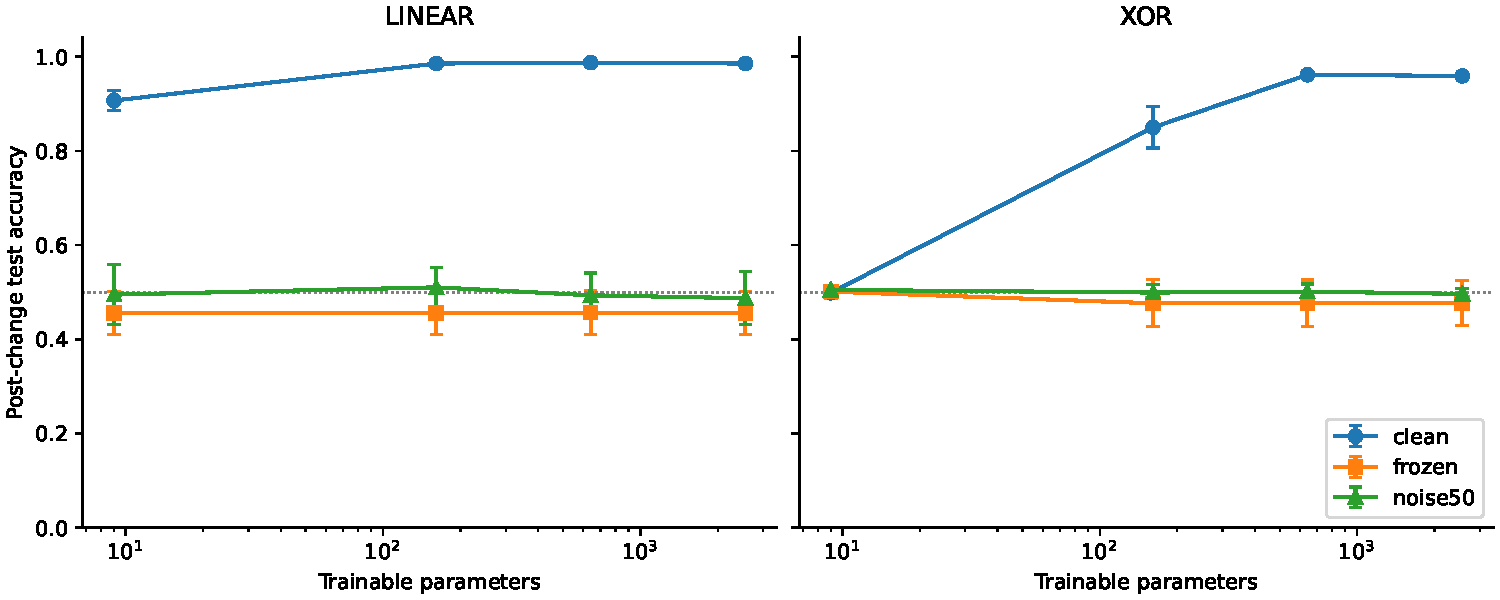
\includegraphics[width=\textwidth]{results/study-a-v2/capacity-feedback.pdf}
\caption{Capacity and feedback jointly determine observed accuracy. Error
bars are descriptive 95\% t intervals across 20 seeds. The dotted line is
chance accuracy; noisy feedback can coexist with information retained from
warmup, so individual noisy outcomes need not equal chance.}
\end{figure}

At an equal adaptation arithmetic proxy, the small model's 256 updates and
the largest model's 16 updates both cost 7,077,888 proxy FLOPs. The small
model leads by 42.80 points on linear tasks and 34.72 on XOR. However, it
receives sixteen times as many new examples, while the large model's warmup
cost is sixteen times greater. This is a particular compute/information trade,
not an isolated causal effect of feedback-loop efficiency or a scaling law.

\subsection{Feedback variations, transfer, and retention}
For the 161-parameter model, clean, 25\% corruption, and 50\% corruption yield
98.53\%, 92.05\%, and 51.03\% accuracy on linear tasks and 84.97\%, 71.84\%,
and 49.92\% on XOR. Inverted feedback yields 1.20\% and 13.32\% respectively.
More updates can reinforce the wrong target when the update rule assumes
trusted labels.

Delayed feedback reaches 98.28\% and 81.87\% at the online endpoint. After
flushing, its scores and final training losses equal clean feedback for every
seed and capacity. This equality is a correctness check for ordered updates,
not an additional empirical discovery about latency.

\begin{figure}[ht]
\centering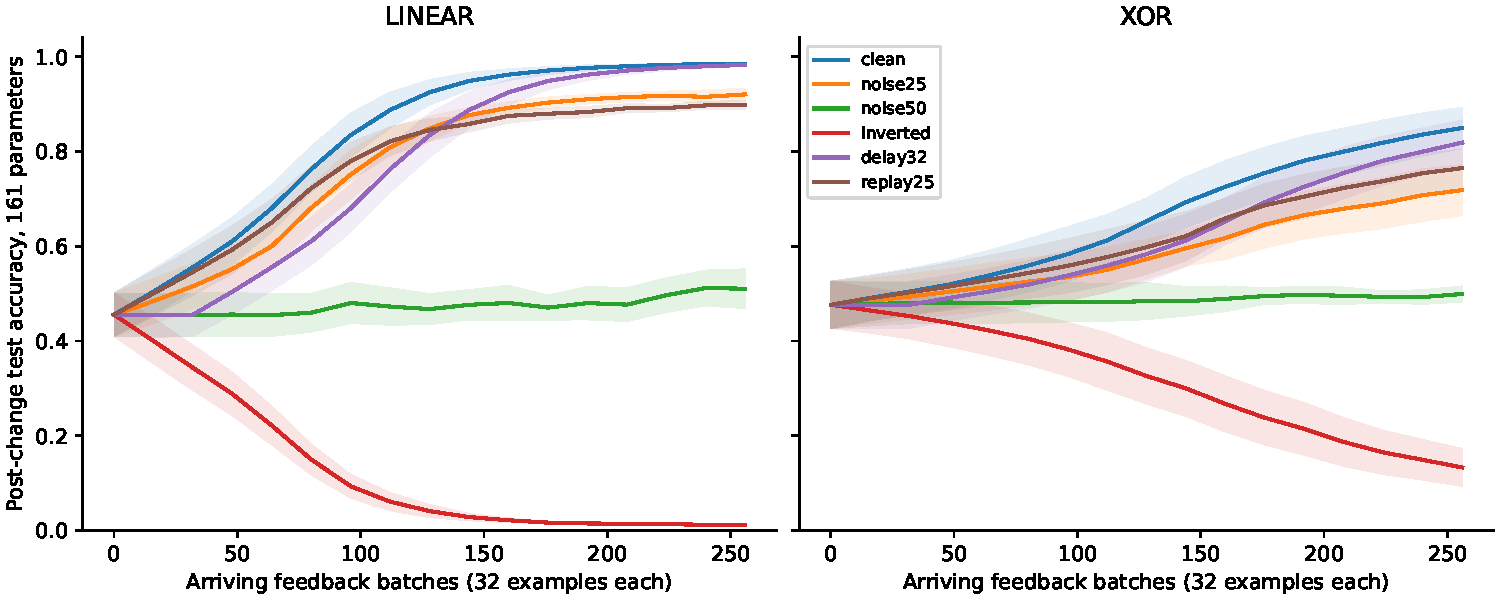
\includegraphics[width=\textwidth]{results/study-a-v2/learning-curves.pdf}
\caption{The same 161-parameter learner under six update conditions. Shading
shows descriptive 95\% seed-level intervals at fixed arrival checkpoints.}
\end{figure}

Clean small-model uniform-input accuracy is 98.44\% for linear rules and
88.19\% for XOR. This is distribution transfer within the same known rule
family, not transfer to an unrelated task. Old-rule accuracy after clean
adaptation is 45.23\% and 51.94\%. Replay raises these to 54.92\% and
64.43\% while lowering new-rule accuracy to 89.85\% and 76.48\%.
Because rules may conflict without a task identifier, this is an adaptation--
retention tradeoff; perfect performance on both is not always possible.

\subsection{Study B: feedback does not guarantee compositional gains}
\begin{table}[ht]
\centering
\caption{Study B mean constrained first-token accuracy (\%), 24 environments.
Direct tests use one command; composition tests use two. Chance is 12.5\%.}
\begin{tabular}{l r r r r r}
\toprule
Model & Direct none & Direct clean & Compose none & Compose clean & Compose oracle\\
\midrule
0.5B & 13.80 & 12.24 & 11.46 & 11.46 & 11.46\\
1.5B & 13.28 & 13.02 & 11.20 & 12.63 & 12.89\\
3B & 10.16 & 5.73 & 13.02 & 12.63 & 14.32\\
7B & 13.80 & 26.56 & 13.80 & 17.58 & 26.82\\
\bottomrule
\end{tabular}
\end{table}

For the primary 0.5B comparison, clean feedback and self-generated examples
both yield 11.46\% composition accuracy. The paired difference is 0.00 points
(95\% t CI [-1.03,1.03]; bootstrap [-0.78,1.04]). Clean-minus-none is also
0.00 points. This is a failure to demonstrate the hypothesized gain with this
mechanism, not proof that every feedback mechanism must fail.

The 7B model reaches 26.56\% on direct tasks with clean-16 examples versus
13.80\% without examples. Its composition scores are 17.58\% and 13.80\%,
respectively: a descriptive paired difference of 3.78 points (95\% CI
[0.38,7.17]). With explicit offsets, direct accuracy rises to 75.52\%, while
composition reaches 26.82\%. Representation of the instruction, inference of
the latent rule, and execution of compositions are distinct bottlenecks.

\begin{figure}[ht]
\centering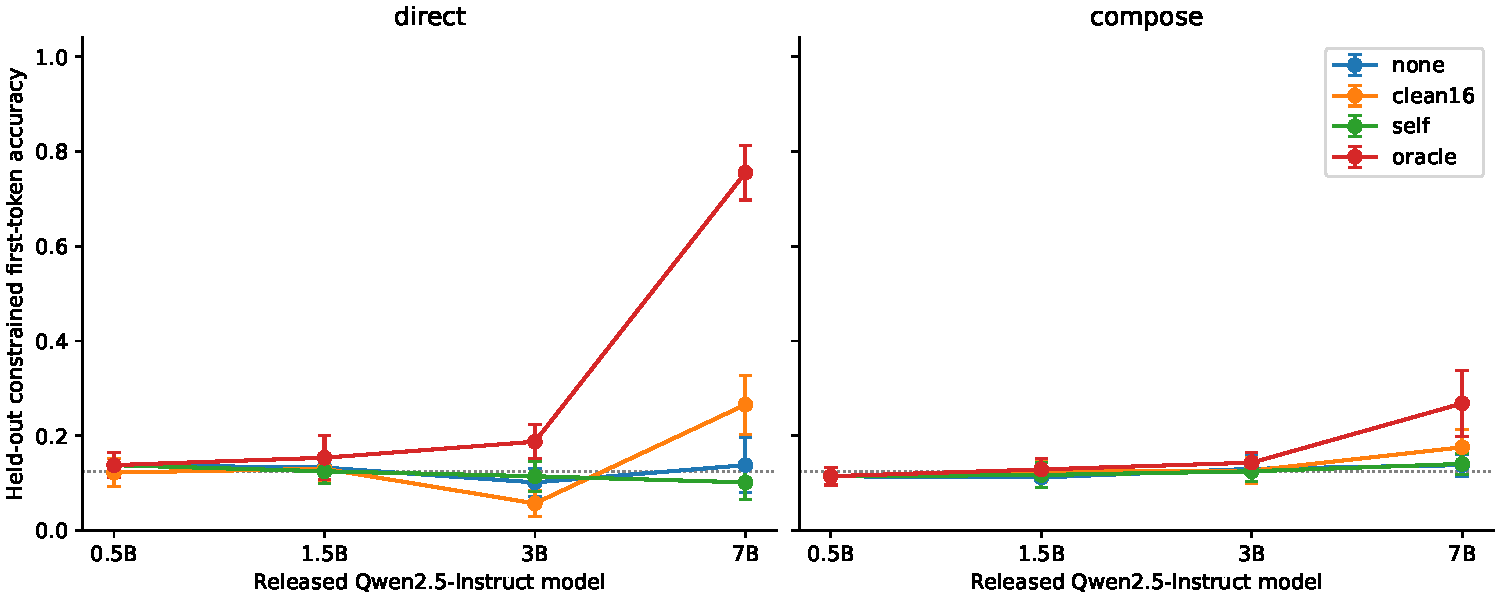
\includegraphics[width=\textwidth]{results/study-b-v1/language-model-feedback.pdf}
\caption{Released-model size and the supplied evidence affect direct and
compositional performance differently. Error bars are descriptive environment-
level 95\% t intervals. The oracle provides extra structured information;
it is not a cost-matched competitor.}
\end{figure}

LoRA trains 540,672 parameters in addition to the frozen 0.494B base. Without
example context, its direct accuracy is 26.30\% versus 13.80\% for the base.
The paired direct gain is 12.50 points (descriptive 95\% t CI [3.76,21.24]).
Composition accuracy is 13.15\%; its paired improvement over no-feedback base
is 1.69 points (95\% CI [-2.12,5.50]). Retaining examples at inference yields
13.28\% composition accuracy but reduces direct accuracy to 9.90\%.
Thus the persistent single-command gain is strongly context-dependent:
adding the same demonstrations does not preserve it. These results distinguish
a gain under the training prompt format from robust compositional transfer.

Each frozen-model suite processes 2,156,304 unpadded input tokens in 888
forward calls, including self-history construction and evaluation. Measured
suite times are 21.81, 56.22, 109.02, and 234.69 seconds; peak allocated memory
is 1.20, 3.41, 6.41, and 15.29 GiB. These figures are whole-suite accounting,
not equal lifetime budgets or per-condition causal estimates. The LoRA suite
adds 1,486,848 training input tokens and 86.67 measured update seconds. Its
extra optimization is explicitly not cost-matched to frozen inference.

\subsection{Study C: format and budget limit the generation comparison}
All 9,216 held-out predictions and 768 self-history records per model pass
source, model-revision, environment, completeness, raw-token decoding, and
score checks. Table~\ref{tab:c} reports composition accuracy; Figure~\ref{fig:c}
also shows direct predictions.

\begin{table}[htbp]
\centering\small
\begin{tabular}{llrrrr}
\toprule
Model & Interface & No examples & Clean 16 & Self & Oracle \\
\midrule
0.5B & First token & 10.68 & 11.20 & 10.68 & 10.68 \\
0.5B & Generation & 0.00 & 0.00 & 0.00 & 0.00 \\
7B & First token & 13.15 & 16.15 & 12.24 & 24.74 \\
7B & Generation & 0.00 & 6.90 & 0.26 & 97.27 \\
\bottomrule
\end{tabular}
\caption{Study C composition accuracy (\%). Generation scores include invalid
and truncated responses as defined by the frozen parser; they must be read
with the format and budget results below.}
\label{tab:c}
\end{table}

The primary 0.5B interaction is $-0.52$ percentage points (95\% t interval
[$-1.16$,0.11]; bootstrap [$-1.17$,0.00]). Its first-token clean-minus-none
effect is 0.52 points, while the generation effect is exactly zero in this
sample. Every generated answer is the literal \texttt{N} followed by EOS,
including the oracle condition. This is a failure of the tested instructions
and output interface; it cannot establish that the model lacks the reasoning
capacity measured by a different interface.

For 7B, oracle generation reaches 100\% direct and 97.27\% composition
accuracy, compared with 69.53\% and 24.74\% under first-token scoring. Thus the
narrow first-token interface can substantially understate execution capability
when the true rules are supplied. With examples, generation's clean-minus-none
composition contrast is 6.90 points (descriptive 95\% interval [4.04,9.76]),
but absolute clean accuracy falls from 16.15\% to 6.90\%. Generation improves
that contrast partly against a control with zero measured accuracy; it does
not establish a superior overall inference method.

The 128-token cap is material. In 7B composition queries, truncation rates are
100\%, 88.28\%, 95.70\%, and 0.26\% for no examples, clean examples, self
examples, and oracle offsets respectively. Corresponding invalid-format rates
are 100\%, 88.28\%, 95.57\%, and 0.26\%. A truncated response can still contain
a parseable final line, so these quantities need not coincide. Clean-example
direct generation scores 24.22\%, with 57.55\% truncation. These outcomes
leave longer-budget example induction unresolved; they are not evidence of an
unrestricted inability to infer the offsets.

Self-history also deteriorates under the interface: all 384 generated examples
for 0.5B and 354 of 384 for 7B are invalid. The resulting histories contain the
literal \texttt{invalid}, as specified. They are not 16 valid critiques or
error-directed repairs. The contrast measures the complete construction of this
self-history under the fixed prompt and budget.

Whole-suite elapsed times, excluding loading, are 28.92 and 1,831.46 seconds.
Each model uses 672 calls per interface, including history acquisition. The 7B
first-token and generation paths take 133.83 and 1,695.16 measured forward
seconds; generation emits 554,021 tokens, or 599,945 token slots with batch
padding. Such costs are recorded, not matched. All generation defaults,
including the model-specific repetition penalties, remain part of the treatment.

\begin{figure}[htbp]
\centering
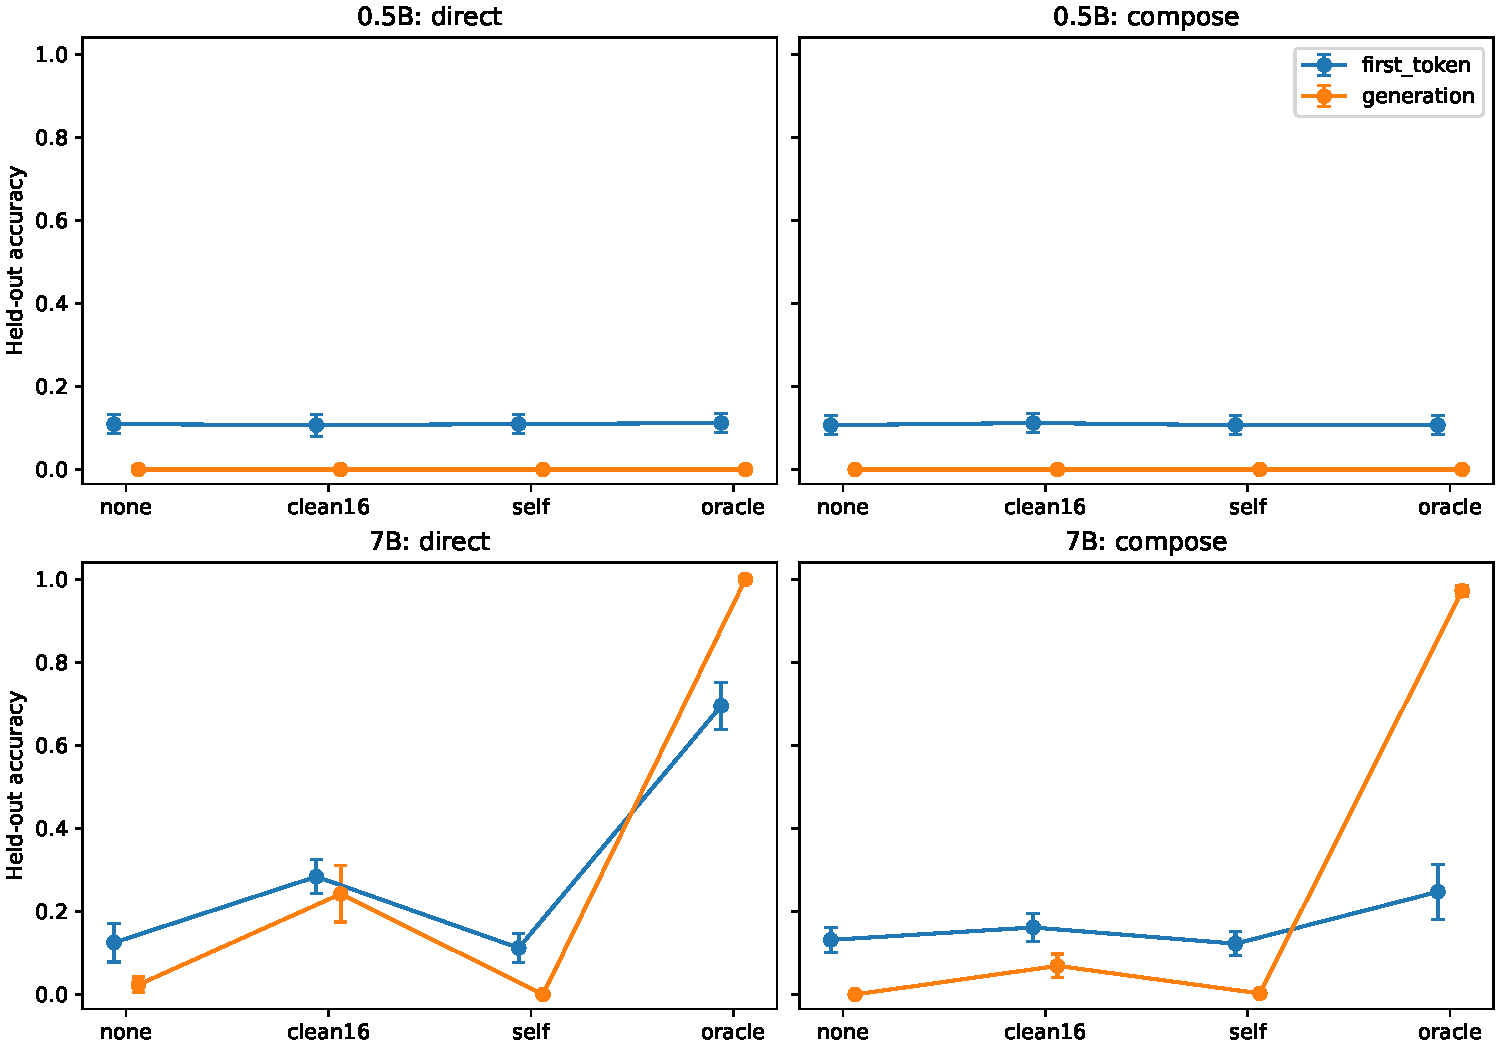
\includegraphics[width=\linewidth]{results/study-c-v1/generation-interface.pdf}
\caption{Study C response interfaces. Error bars are descriptive 95\% intervals
across 24 environment means. Strong oracle execution under generation coexists
with pervasive format or token-cap failures in other conditions.}
\label{fig:c}
\end{figure}

\subsection{Study D: longer continuations recover example-based performance}
All 3,456 continuations and 216 actual generation batches pass the registered
integrity checks. Table~\ref{tab:d} and Figure~\ref{fig:d} compare paired
prefixes on the same 24 new environments.

\begin{table}[htbp]
\centering\small
\begin{tabular}{lrrrr}
\toprule
& \multicolumn{2}{c}{Direct} & \multicolumn{2}{c}{Composition} \\
Condition & 128 tokens & 512 tokens & 128 tokens & 512 tokens \\
\midrule
No examples & 3.12 & 11.98 & 0.00 & 14.06 \\
Clean 16 & 20.05 & 59.90 & 7.94 & 70.57 \\
Oracle offsets & 100.00 & 100.00 & 96.61 & 96.88 \\
\bottomrule
\end{tabular}
\caption{Study D accuracy (\%) with fixed instructions and model. Shorter
scores use prefixes of the same deterministic continuations.}
\label{tab:d}
\end{table}

The primary clean composition difference is 62.63 percentage points (95\% t
interval [56.10,69.16]; bootstrap [56.38,68.75]). The clean-minus-none effect
at 512 tokens is 56.51 points (descriptive 95\% interval [48.99,64.03]),
compared with 7.94 at 128 tokens. The control also improves as its answers
become complete. Thus the larger budget reveals a substantial measured benefit
from the correct examples under this fixed interface.

Clean composition truncation falls from 87.76\% to 3.26\%, and invalid-format
rate falls from 87.76\% to 2.99\%. Among 768 clean composition queries, 481
change from wrong to correct and none change in the opposite direction. All
481 gains occur where the shorter prefix was invalid. Accordingly, this result
does not show correction of 481 previously valid wrong answers or isolate a
reasoning mechanism from completion of the requested answer format. It shows
that early evaluation of an unfinished response can seriously understate the
model's use of existing information. No additional environmental feedback
arrives during these continuations.

Oracle composition changes little, from 96.61\% to 96.88\%, while clean direct
accuracy rises from 20.05\% to 59.90\%. These separate direct and composition
query sets have different input lengths and generated traces; their ordering
is not a general statement that composition is easier than direct prediction.
The experiment adds no persistence across tasks, active exploration, or new
parameter updates. It neither resolves small-model format failures nor
establishes an advantage of a small learner over a large one.

The run takes 1,436.61 seconds, including 1,435.81 measured generation seconds,
processing 853,632 input tokens and 654,495 output tokens. Output padding raises
token slots to 1,044,320. The shorter prefixes have no separately measured
wall times, so these records do not support a 128-versus-512 speed ratio.

\begin{figure}[htbp]
\centering
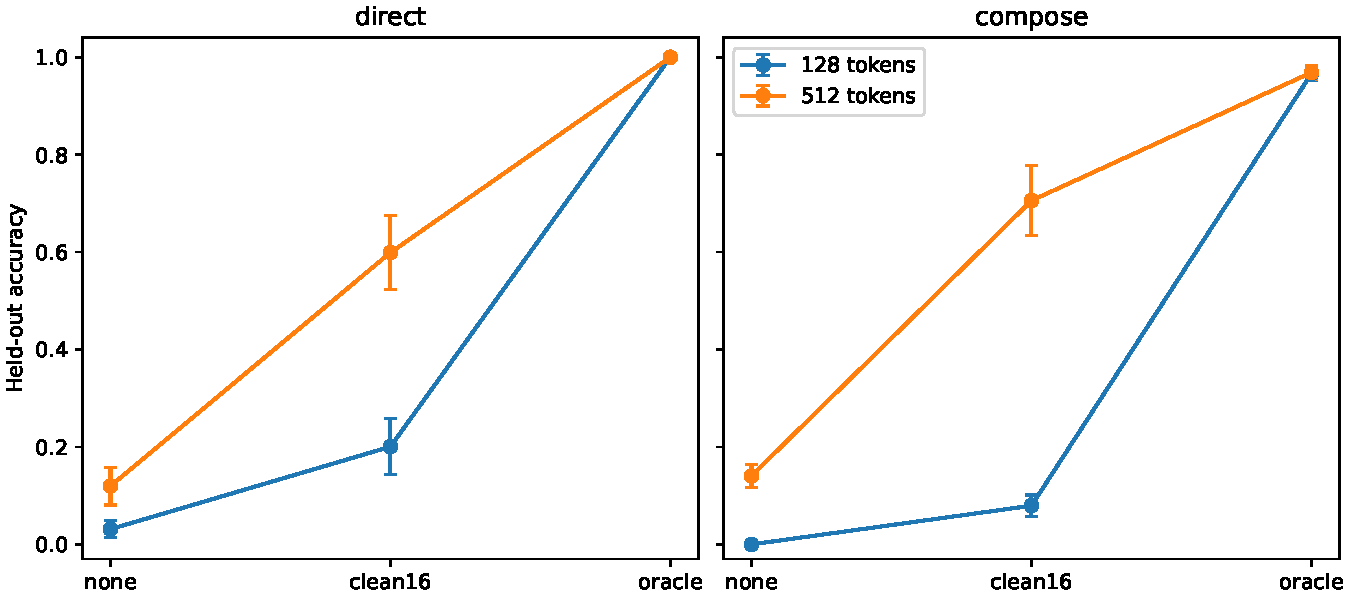
\includegraphics[width=\linewidth]{results/study-d-v1/generation-budget.pdf}
\caption{Study D generation budgets. Error bars are descriptive 95\% intervals
across 24 environment means. Extending the same continuation substantially
changes example-based accuracy; oracle execution is already nearly complete
at the shorter budget.}
\label{fig:d}
\end{figure}

\subsection{Study E: one-pass updates do not establish retained gains}
The complete 24-environment run passes all grid, source, model, prompt,
feedback-order, state-reset, and adapter-file checks. Table~\ref{tab:e} shows
final accuracy; Figure~\ref{fig:e} reports the fixed checkpoint curves.

\begin{table}[htbp]
\centering\small
\begin{tabular}{lrr}
\toprule
Condition & Direct & Composition \\
\midrule
No feedback & 14.06 & 14.32 \\
Context after 16 outcomes & 12.50 & 14.45 \\
Per-outcome LoRA & 13.28 & 13.67 \\
Error-only LoRA & 10.68 & 11.98 \\
Per-outcome LoRA with context & 5.47 & 13.54 \\
Error-only LoRA with context & 5.99 & 12.89 \\
\bottomrule
\end{tabular}
\caption{Study E constrained first-token accuracy (\%). Adapter-only rows
remove the correct transcript at evaluation. Chance is 12.5\%.}
\label{tab:e}
\end{table}

The primary per-outcome composition change is $-0.65$ percentage points.
Its 95\% t interval is [$-4.04$, 2.74]; the bootstrap interval is
[$-3.78$, 2.47]. Of 768
composition queries, 99 change from wrong to correct and 104 change from
correct to wrong. The updates change behavior without demonstrating a net
gain. Error-only updating has a descriptive change of $-2.34$ points
(95\% interval [$-5.53$,0.85]), with 86 improvements and 104 regressions.
Context alone changes composition accuracy by 0.13 points
([$-0.34$,0.60]). These intervals describe uncertainty under this protocol;
a null result is not a proof of no possible feedback benefit.

Adding the correct transcript to the per-outcome adapter lowers direct
accuracy from 13.28\% to 5.47\%, a descriptive paired difference of $-7.81$
points (95\% interval [$-12.16$,$-3.46$]). The error-only adapter falls from
10.68\% to 5.99\% ($-4.69$ points; [$-8.67$,$-0.70$]). This repeats the
qualitative context dependence seen in Study B; it does not establish that
context is generally harmful. Neither tested update rule yields a demonstrated
composition improvement under this short adaptation schedule and interface.

The suite takes 72.80 seconds after model loading, recording 24,192 evaluation
rows in 1,512 batches and 1,152 pre-update prediction calls. Per-outcome LoRA
applies 384 updates across environments, processing 46,464 optimization input
tokens in 7.82 measured seconds. Error-only LoRA applies 337 updates with
40,777 tokens in 6.82 seconds. Whole-suite peak allocation is
1,305,673,728 bytes. Full per-condition inference, padding, and update costs
are archived. These are unequal adaptation costs, not lifetime compute estimates.

\begin{figure}[htbp]
\centering
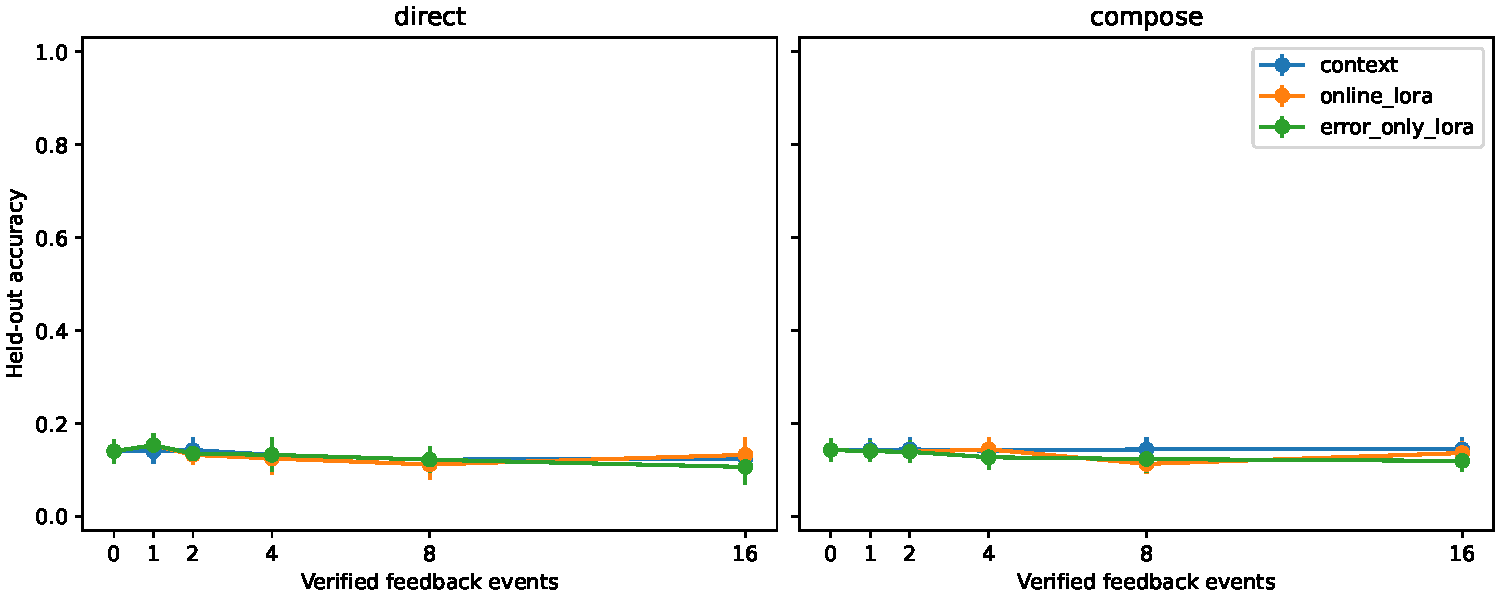
\includegraphics[width=\linewidth]{results/study-e-v1/online-feedback.pdf}
\caption{Study E fixed checkpoints. Error bars are descriptive 95\% t intervals
across 24 environments. Repeated verified outcomes do not produce demonstrated
final compositional gains with either tested adapter update rule.}
\label{fig:e}
\end{figure}

\subsection{Study F: external checks do not establish a reliable gain}
Both model suites pass the full audit of 120 proposals, 120 rule files,
and 5,760 held-out evaluations each. Table~\ref{tab:f} reports the initial and
final proposals; Figure~\ref{fig:f} includes both fixed revisions. Every
proposal terminates at EOS before the 512-token cap.

\begin{table}[htbp]
\centering\small
\begin{tabular}{llrrrr}
\toprule
Model & Proposal & Direct & Composition & Valid/24 & Exact/24 \\
\midrule
0.5B & Initial & 11.46 & 9.38 & 18 & 0 \\
& Self-review final & 11.46 & 9.38 & 18 & 0 \\
& Checked final & 10.42 & 13.41 & 17 & 0 \\
7B & Initial & 51.04 & 43.23 & 21 & 4 \\
& Self-review final & 52.08 & 42.32 & 22 & 3 \\
& Checked final & 54.17 & 45.44 & 21 & 6 \\
\bottomrule
\end{tabular}
\caption{Study F executor accuracy (\%) and rule counts. Invalid rules score
zero. The stored rules supply offsets; a human-provided algorithm executes
the held-out queries. Results measure the combined system.}
\label{tab:f}
\end{table}

The primary 0.5B checked-minus-self composition effect is +4.04 percentage
points (95\% t CI [$-2.78$,10.85]; bootstrap [$-1.56$,11.07]). Neither interval
demonstrates a positive effect under this protocol. Checked-minus-initial has
the same mean and t interval. Self-review has zero net composition change,
with two query answers gained and two lost. Against self-review, checked
revision gains 60 composition answers and loses 29, while direct accuracy
falls by 1.04 points (CI [$-10.11$,8.02]). No 0.5B proposal recovers all four
offsets at any stage; the final 0/24 exact-recovery rate has Wilson 95\% CI
[0.00\%,13.80\%]. Thus lack of observed recovery is not a universal zero-rate
claim.

For 7B, comparing checked review with self-review gives a composition difference
of +3.13 points (CI [$-9.32$,15.57]). The change from the initial proposal is
+2.21 points (CI [$-9.93$,14.36]). Checked revision recovers two previously incorrect rule
vectors and retains all four initially correct vectors. Self-review loses one
initially correct vector and gains none. Final exact recovery is 6/24
(25.00\%, Wilson CI [12.00\%,44.90\%]) versus 3/24
(12.50\%, CI [4.34\%,31.00\%]); these are descriptive rates, not a confirmed
between-arm effect. Against the initial proposal, checked review gains 81
composition answers and loses 64. Partial rule changes can therefore cause
many answer regressions even when exact-vector retention appears stable.

The supplied symbolic estimator identifies all languages and executes all
held-out targets correctly. No observed nonexact proposal has perfect
composition accuracy, although the algebraic +4 counterexample remains valid.
Valid saved rules occupy 34 bytes each, including syntax and newline. This
compact representation demonstrates externally supplied persistence and
execution, not neural retention or a new memory mechanism.

Validity remains an interface limitation. Across all five stages, all 32
invalid 0.5B proposals contain repeated offsets. Of 12 invalid 7B proposals,
nine use negative offsets outside the required 0--7 range, two contain
malformed JSON, and one repeats an offset. Seed 8012's final checked rule
is semantically exact with $-1\equiv7\pmod8$, but the frozen interface scores
it as invalid. We do not normalize scores after collection. Unlike Study C,
most proposals satisfy the new interface, but rule correctness remains weak.

Each model uses ten actual generation batches. Whole-suite unpadded input
and output token counts are 51,427/4,680 for 0.5B and 50,283/3,305 for 7B.
Generation takes 2.724 and 12.457 seconds, with runner totals of 2.763 and
12.497 seconds after loading; peak allocation is 1.269 and 15.546 GiB.
Diagnostic checking of all proposals takes 0.00114 and 0.00123 seconds.
These costs count shared initial generation once and exclude offline scoring
and plotting. Matching revision counts does not match measured inference cost
or the models' pretraining investment.

\begin{figure}[htbp]
\centering
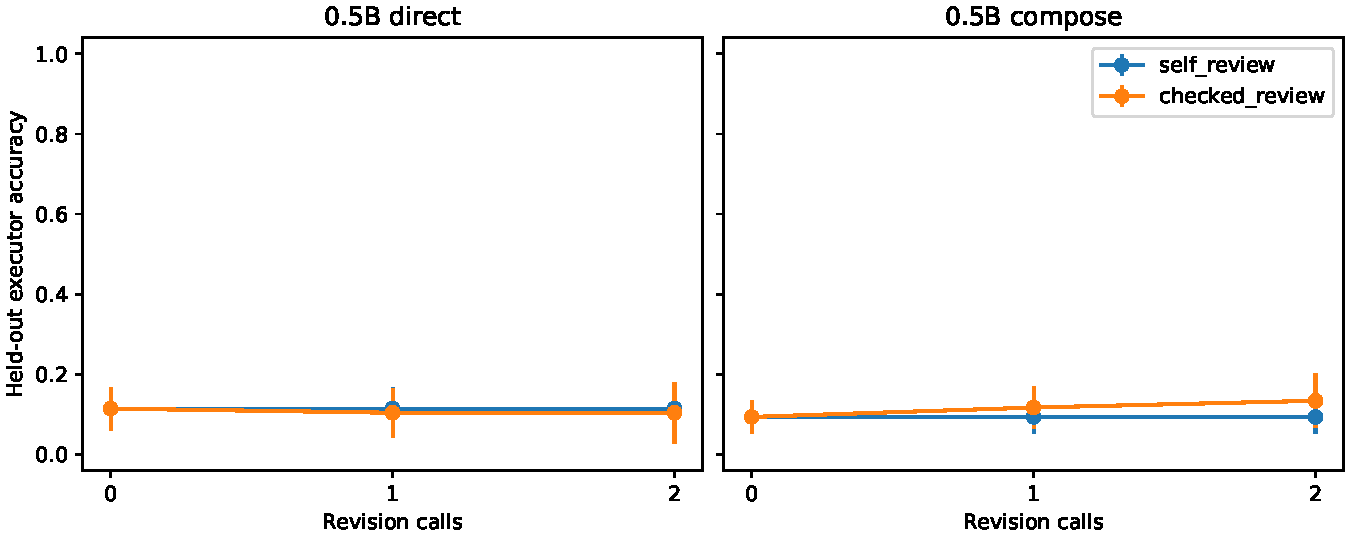
\includegraphics[width=\linewidth]{results/study-f-v1/formal-0.5B-v1/rule-revision.pdf}
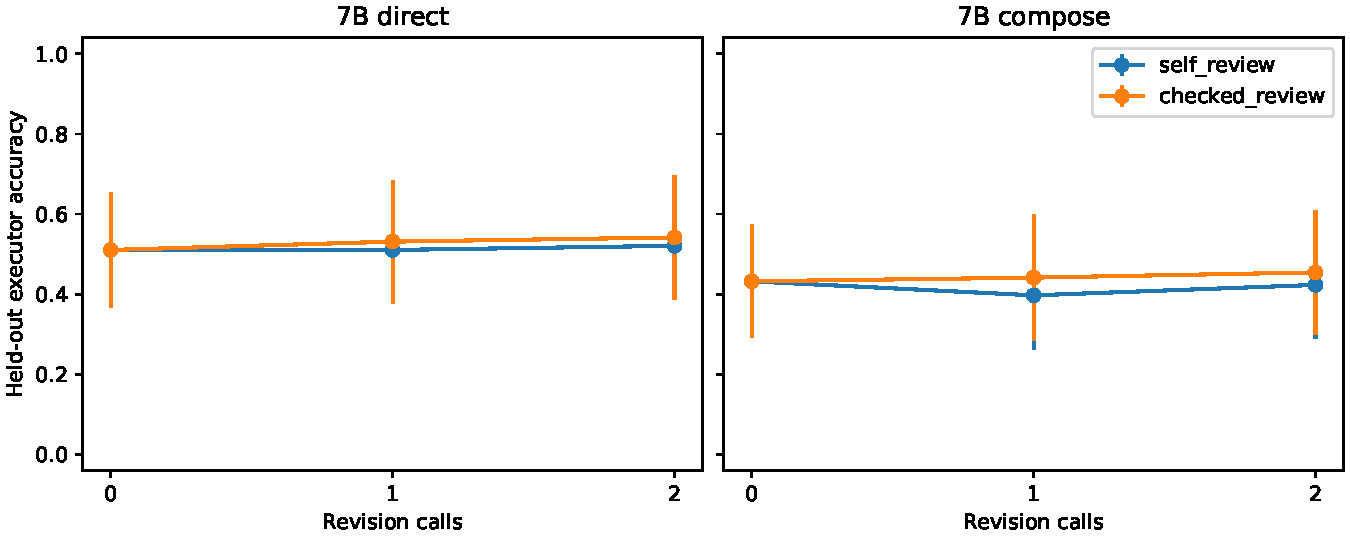
\includegraphics[width=\linewidth]{results/study-f-v1/formal-7B-v1/rule-revision.pdf}
\caption{Study F held-out execution from saved rules. Error bars are descriptive
95\% t intervals over 24 environments. The two branches share the initial
proposal; all revisions run and the final proposal is scored.}
\label{fig:f}
\end{figure}

\subsection{Study G: longer history does not establish cumulative improvement}
Both model suites pass the audit of 1,584 proposals, 1,584 saved rules,
and 76,032 held-out evaluations each. All 3,188 transferred manifest entries
match. The first-revision inputs and outputs are identical across branches,
and every proposal terminates at EOS before the cap. Table~\ref{tab:g}
reports final outcomes; Figure~\ref{fig:g} retains all declared checkpoints.

\begin{table}[htbp]
\centering\small
\begin{tabular}{llrrrr}
\toprule
Model & Proposal & Direct & Composition & Valid/48 & Exact/48 \\
\midrule
0.5B & Initial & 13.54 & 13.02 & 44 & 0 \\
& Last only, revision 16 & 10.42 & 7.94 & 32 & 0 \\
& Full history, revision 16 & 10.42 & 7.23 & 30 & 0 \\
7B & Initial & 53.13 & 39.52 & 45 & 4 \\
& Last only, revision 16 & 47.40 & 34.51 & 44 & 5 \\
& Full history, revision 16 & 47.92 & 36.65 & 41 & 9 \\
\bottomrule
\end{tabular}
\caption{Study G executor accuracy (\%) and rule counts over 48 environments.
Each branch makes 16 checked revisions from a shared initial proposal.
Invalid rules score zero; no earlier candidate replaces the final proposal.}
\label{tab:g}
\end{table}

The primary 0.5B full-history-minus-last-only direct effect is 0.00 percentage
points (95\% t CI [$-3.96$,3.96]; bootstrap [$-3.65$,3.65]). The zero mean
combines 20 wrong-to-correct and 20 correct-to-wrong answer differences;
it does not mean that the two branches produce identical outcomes. Both finish
3.13 points below initial direct accuracy (last-only CI [$-8.01$,1.76];
full-history CI [$-8.23$,1.98]). No small-model proposal recovers an exact
rule at any stage; each final 0/48 rate has Wilson CI [0.00\%,7.41\%].
The secondary composition changes from initial are $-5.08$ points for last
only (CI [$-9.22$,$-0.94$]) and $-5.79$ for full history
(CI [$-10.04$,$-1.55$]). These descriptive intervals receive no multiplicity
adjustment and do not replace the primary endpoint. The between-branch
composition difference is $-0.72$ points (CI [$-2.84$,1.41]).

For 7B, the descriptive direct contrast is +0.52 points
(CI [$-11.69$,12.73]); composition is +2.15 (CI [$-9.55$,13.85]).
Direct changes from initial are $-5.73$ points for last only
(CI [$-13.54$,2.09]) and $-5.21$ for full history (CI [$-16.31$,5.89]).
Final exact recovery is 5/48 (10.42\%, Wilson CI [4.53\%,22.17\%]) versus
9/48 (18.75\%, CI [10.19\%,31.94\%]); these marginal rates do not establish
a between-branch effect. Last only gains two exact rules and loses one
relative to the four initially exact rules. Full history gains eight but
loses three, retaining only one of the four. Higher final exact recovery
therefore does not imply stable retention of initial successes. Relative to
initial direct answers, last only gains 48 and loses 92; full history gains
88 and loses 128.

Repeated proposals remain common. Each arm has 768 transitions nested in 48
environments. In 0.5B, 483/522 current valid-wrong last-only proposals and
436/485 full-history proposals have appeared earlier in their respective
branches. The corresponding invalid-proposal counts are 231/246 and 262/283.
Among valid-to-valid pairs, last only gains 11 correct offsets and loses nine;
full history gains 37 and loses 32. These component counts exclude invalid
transitions and cannot account for complete score changes alone. For 7B,
previously seen valid-wrong proposals occur in 525/603 last-only and 425/525
full-history transitions; previously seen exact proposals occur in 98/104
and 146/159. Repetition of correct behavior differs from repeating an error.
These nested descriptive counts do not establish permanent cycles or make
reduced repetition a proxy for learning.

Actual suite input/output tokens are 1,244,712/61,776 for 0.5B and
1,168,726/44,253 for 7B. Generation takes 41.294 and 227.323 seconds;
post-loading runner totals are 42.085 and 228.098 seconds, with peak
allocations of 2.380 and 19.485 GiB. Standalone input tokens, initial included, are
367,542 versus 894,642 in 0.5B and 360,150 versus 826,048 in 7B for last
only versus full history: ratios of 2.43 and 2.29. Accounted generation times
are 15.836 versus 26.315 seconds and 78.413 versus 152.625 seconds. These
totals reuse the measured shared-initial cost, not separately timed reruns.
Full history increases measured cost without establishing a direct-accuracy
benefit in these 16 revisions.

\begin{figure}[htbp]
\centering
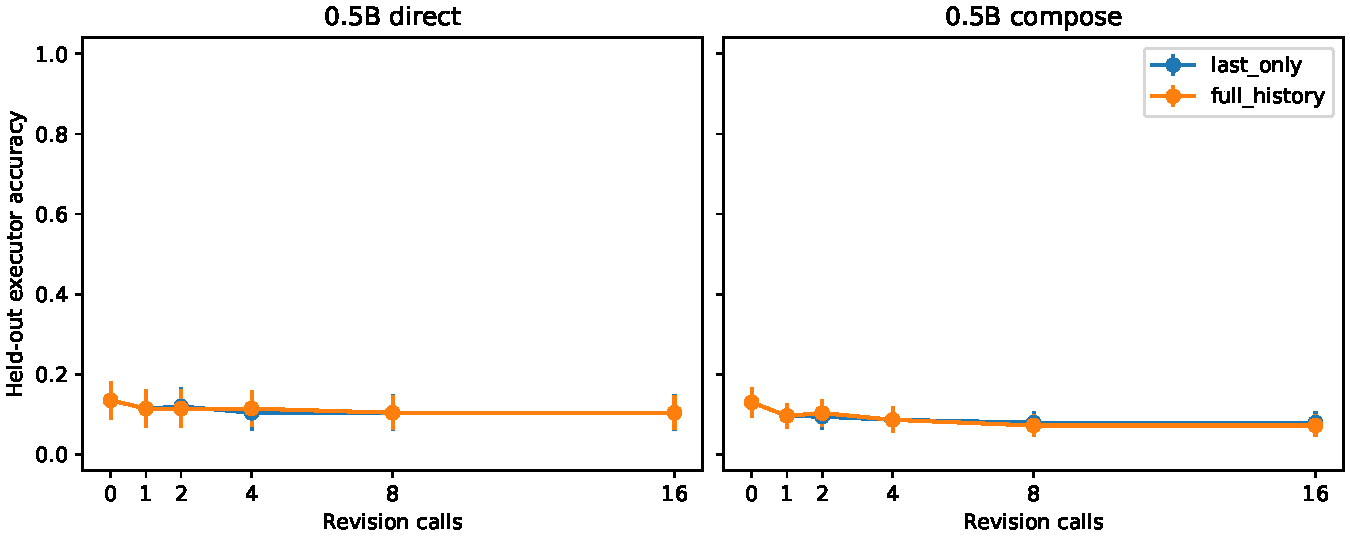
\includegraphics[width=\linewidth]{results/study-g-v1/formal-0.5B-v1/feedback-history.pdf}
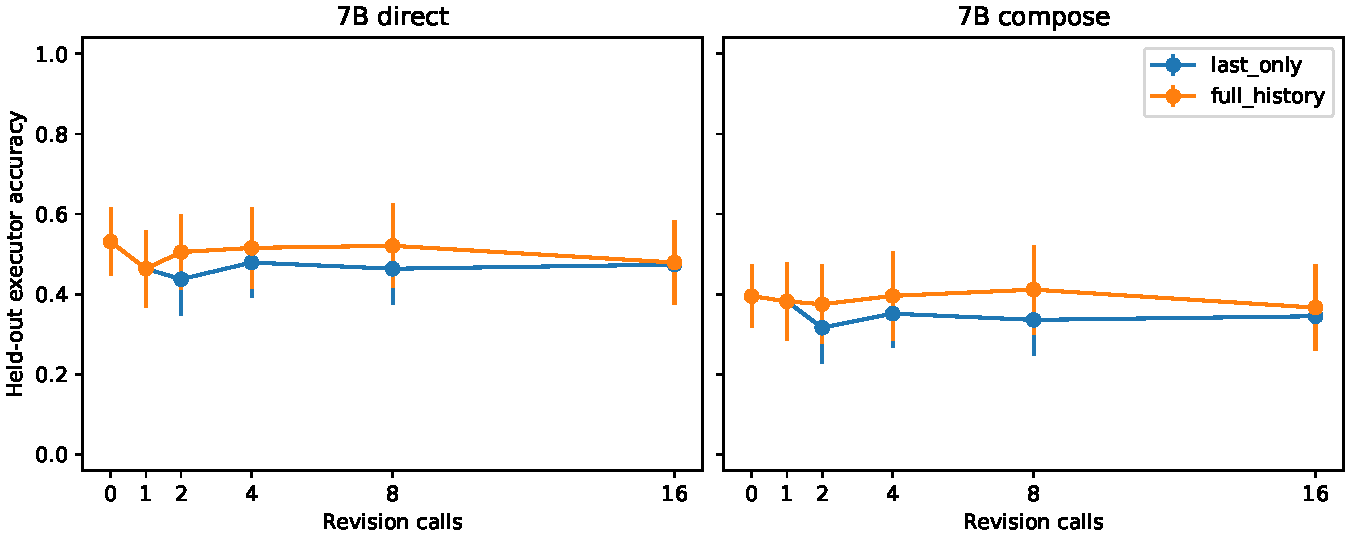
\includegraphics[width=\linewidth]{results/study-g-v1/formal-7B-v1/feedback-history.pdf}
\caption{Study G held-out execution at the prespecified checkpoints. Error
bars are descriptive 95\% t intervals over 48 environments. Both branches
share the initial rule and have identical first-revision computation; all 16
revisions run without an acceptance gate.}
\label{fig:g}
\end{figure}

\subsection{Exploratory selection and uniform-proposal references}
After reviewing Study G and freezing manuscript v8, we specify a post-hoc
analysis of its fixed candidate pools. At each declared checkpoint, an
external selector scores every valid candidate against all 16 disclosed
examples and keeps the earliest maximum in the available prefix. Invalid
proposals rank below valid ones, including valid zero-score rules; an
all-invalid prefix retains its initial invalid proposal. No later candidate,
hidden queries or their targets, or true offset vector enters selection. No new model
call occurs, and the original final-proposal endpoints remain unchanged.

For this known additive family, each command has four training and four
disjoint direct-test inputs. A wrong offset fails every input for its command,
so training accuracy equals direct accuracy for every valid rule; both scores
are zero for invalid rules. Selection therefore guarantees nondecreasing
direct accuracy over prefixes by construction. This is a supplied algorithmic
property, not evidence of neural learning or transfer to a different family.
Composition has no corresponding guarantee because of the +4-offset alias.

Table~\ref{tab:selection} distinguishes final proposals from selected
candidates. The 7B last-only pools contain exact valid rules in 10 environments
and the full-history pools in 17. The final proposals discard five and eight
of these exact solutions, respectively. In contrast, none of the 0.5B pools
contains an exact valid rule for selection to retrieve. Per-environment direct
scores improve in 10, 13, 20, and 22 environments in table order, with none
decreasing. Individual direct answers can still regress when the retained
rule has a different subset of correct offsets: gained/lost counts are 60/4,
76/8, 132/8, and 172/0. Composition scores decrease in 5, 4, 2, and 3
environments despite higher group means. Selection retains existing candidates;
it cannot predict what a model would generate if an acceptance gate changed
later prompts or feedback.

\begin{table}[htbp]
\centering\small
\begin{tabular}{llrrrrrr}
\toprule
& & \multicolumn{3}{c}{Direct accuracy (\%)} & \multicolumn{3}{c}{Exact count / 48} \\
\cmidrule(lr){3-5}\cmidrule(lr){6-8}
Model & Pool & Final & Selected & Uniform & Final & Selected & Uniform \\
\midrule
0.5B & Last only & 10.42 & 17.71 & 48.47 & 0 & 0 & 0.46 \\
& Full history & 10.42 & 19.27 & 48.47 & 0 & 0 & 0.46 \\
7B & Last only & 47.40 & 63.54 & 63.84 & 5 & 10 & 4.42 \\
& Full history & 47.92 & 70.31 & 63.84 & 9 & 17 & 4.42 \\
\bottomrule
\end{tabular}
\caption{Post-hoc Study G descriptions. Final and selected columns are
observed outcomes. Uniform columns are exact expectations for 16 independent
uniform legal proposals after the same observed neural initial rule, followed
by training-example selection. They are not observed random-agent runs or
confidence bounds. All comparisons include supplied grammar and execution.}
\label{tab:selection}
\end{table}

After viewing these selection outcomes, we specify a second post-hoc
reference: independent uniform legal proposals drawn with replacement and
the same selector. There are $N=8\cdot7\cdot6\cdot5=1680$ legal offset vectors.
Enumeration gives counts $(1001,536,126,16,1)$ for $M=0,1,2,3,4$ correct
positions. An injective relabeling of the eight values maps any legal true
vector to the canonical $(0,1,2,3)$, preserving this distribution. Let
$F(j)=P(M\leq j)$. With $k$ initially correct offsets and $n$ independent
uniform proposals, selected direct accuracy has exact expectation
\[
 \mathbb{E}[A_{\mathrm{direct}}]
 =\frac{1}{4}\left[k+\sum_{j=k+1}^{4}\{1-F(j-1)^n\}\right].
\]
The selected rule is exact with probability one if $k=4$, and otherwise with
probability $1-(1-1/N)^n$. Invalid initial proposals have zero direct score.
We compute exact fractions, using the observed initial training-pass counts
for $k$, without Monte Carlo sampling or a significance claim.

Seventeen uniform proposals without a neural initial call have expected
direct accuracy 48.71\% and exact-rule probability 1.01\%. This uses $k=0$
as a score lower bound and $n=17$; the lower bound is not an additional
candidate. Conditioning instead on each model's shared initial proposal and
adding 16 uniform draws gives Table~\ref{tab:selection}. The 0.5B selected
pools are 30.76 and 29.20 points below that conditional direct expectation.
The 7B last-only pool is 0.30 points below it, while full history is 6.47
points above it. More exact 7B rules coexist with these different direct-score
comparisons. Zero observed exact small-model rules does not establish a rate
below a reference whose expected exact count is only 0.46. These comparisons
describe observed pools relative to policy expectations, not a population
effect or an isolated causal contribution of feedback or model size.

The sampler hardcodes the legal action grammar and always emits valid rules;
its proposals ignore feedback, while the external selector uses all examples.
The conditional reference retains the neural initial call and its prior
learning. Equal candidate opportunities do not match validity, dependence,
checker executions, or measured compute. Selection from recorded pools adds
9,056, 8,464, 12,032, and 11,664 example executions in table order. The
conditional uniform references require 12,992 executions per 0.5B pool group
and 13,008 per 7B group, including valid initial rules. The pure uniform
reference requires 13,056 for 48 environments and no neural initial call.
The two offline analyses take 0.668 and 0.037 seconds before serialization,
excluding imports and original generation. The latter times expectation
calculation, not deployment of random agents. All records and exact fractions
are archived separately from the original formal results.

\subsection{Study H: useful compression and distribution-specific search}
All 768 experience programs are accepted and match their full functions.
The formal suite contains 4,864 searches and separate evaluations, including
4,096 evaluation searches. No accepted evaluation program is a false fit on
the held-out inputs, so exact success and held-out accuracy coincide in this
sample. Unaccepted tasks score zero. This agreement is an observed property,
not a guarantee of the eight-example acceptance rule.

\begin{table}[ht]
\centering
\begin{tabular}{lrrr}
\toprule
Memory & Composition exact & Shifted exact & Definition tokens \\
\midrule
None & 50.39 (258/512) & 50.00 (256/512) & 0 \\
Whole programs & 2.34 (12/512) & 1.17 (6/512) & 4,608 \\
Compressed fragments & 85.16 (436/512) & 9.96 (51/512) & 473 \\
Renamed fragments & 14.65 (75/512) & 12.11 (62/512) & 473 \\
\bottomrule
\end{tabular}
\caption{Study H exact success (\%) at 65,536 primitive operations per task.
Each arm has 16 tasks per family in each of 32 environments. Definition-token
storage is summed over environments and excludes the shared primitive tables
and search implementation. Whole memory has 24 entries per environment;
compressed and renamed memory each have four.}
\label{tab:h}
\end{table}

The prespecified compressed-minus-whole composition contrast is +82.81
percentage points, with a 95\% t interval [77.12,88.51] and percentile
bootstrap interval [77.34,88.09]. Both support a positive effect. All environment
contrasts are positive. This satisfies the declared primary criterion for
this finite intervention. The whole-memory baseline also performs much worse
than no memory: adding complete solutions increases the vocabulary from four
to 28 entries under the fixed breadth-first enumerator. Compressed memory
has eight entries including primitives and exceeds no memory by 34.77 points
on compositions, descriptively. The renamed control has the same number and
lengths of entries but solves only 14.65\%, indicating that entry count and
storage alone do not explain the observed composition performance.

Transfer is distribution-specific. On shifted random programs, compressed
memory solves 9.96\%, compared with 50.00\% without memory. Across the fixed
balanced mixture of both evaluation families, it solves 487/1,024 tasks
versus 514/1,024 without memory. The induced vocabulary changes the search
allocation; it does not remove primitive programs from the policy class.
Reduced success under the cap therefore need not imply loss of representation
or deletion of previously stored knowledge. These are limitations of this
fixed enumeration and representation policy, not evidence that memory is
generally harmful.

Compression reduces the experience encoding from 3,840 primitive tokens to
2,434 corpus tokens plus 473 definition tokens. Experience collection costs
3,110,069 primitive operations, charged to every standalone memory arm.
Including that experience, the aggregate search costs across both evaluation
families are 43.49, 69.10, 42.26, and 63.66 million operations for none,
whole, compressed, and renamed memory. These totals have different success
counts and exclude comparisons, induction, and interpreter overhead; they
are not equal lifetime compute. Compression itself takes 0.833 seconds over
32 environments, with 5,048 candidate-library evaluations. The actual shared
experiment takes 127.832 seconds including journaling on an Intel
Core i5-1135G7 CPU. No neural training or GPU inference occurs in this study.

\subsection{Study I: neural fitting without improved search transfer}
All 768 experience solutions match their full functions and supply 3,840
primitive tokens. The formal run contains 8,960 searches, including 8,192
transfer searches, and 36,864 gradient updates. All 5,761 nonaccepted searches
exhaust their operation cap. No accepted transfer program fails its hidden
evaluation. Thus the observed failure concerns finding a fit under the budget,
with neither a false-acceptance nor an output-format failure in this sample.

\begin{table}[ht]
\centering\small
\begin{tabular}{lrrr}
\toprule
Prior & Neural parameters & Composition exact & Shifted exact \\
\midrule
Uniform & 0 & 50.00 (256/512) & 50.00 (256/512) \\
Counts & 0 & 66.02 (338/512) & 33.59 (172/512) \\
Small frozen & 1,172 & 50.00 (256/512) & 49.80 (255/512) \\
Small trained & 1,172 & 22.85 (117/512) & 10.16 (52/512) \\
Small shuffled & 1,172 & 26.76 (137/512) & 13.67 (70/512) \\
Large trained & 13,892 & 17.58 (90/512) & 9.96 (51/512) \\
Small after 8 attempts & 1,172 & 28.52 (146/512) & 11.91 (61/512) \\
Small after 16 attempts & 1,172 & 23.24 (119/512) & 10.74 (55/512) \\
\bottomrule
\end{tabular}
\caption{Study I exact success (\%) under the same 65,536 primitive-operation
cap per task, with 32 environments and 16 tasks per family per environment.
Parameter counts are per neural model; the count prior instead stores 100
integer cells. Supplied search, verification, tables, and runtime storage are
outside those neural counts. Only the small-trained versus uniform composition
contrast is primary; other rows/comparisons are descriptive.}
\label{tab:i}
\end{table}

The primary contrast is $-27.15$ percentage points. The 95\% t interval is
[$-32.74$, $-21.55$]; the bootstrap interval is [$-32.23$, $-21.68$].
The intervals agree.
Differences are negative in 29 environments, positive in two, and zero in one.
The declared positive prediction fails, with contrary evidence for this
configuration. Identical initial small networks have 50.00\% composition
success when frozen, versus 22.85\% after replay. A larger trained GRU also
has a lower observed score under this schedule; this does not establish a
general capacity optimum or a result about scaling laws.

The simpler count prior has higher observed composition success than uniform
search, 66.02\% versus 50.00\%, but falls to 33.59\% on shifted programs.
Across the balanced mixture it solves 510/1,024 tasks, versus uniform's
512/1,024; small trained solves 169/1,024. We therefore claim no overall
superiority for the count prior. Its use of local sequential structure differs
from both a recurrent learned representation and Study H's callable fragments.
Their storage and algorithms are not capacity-matched.

\begin{figure}[ht]
\centering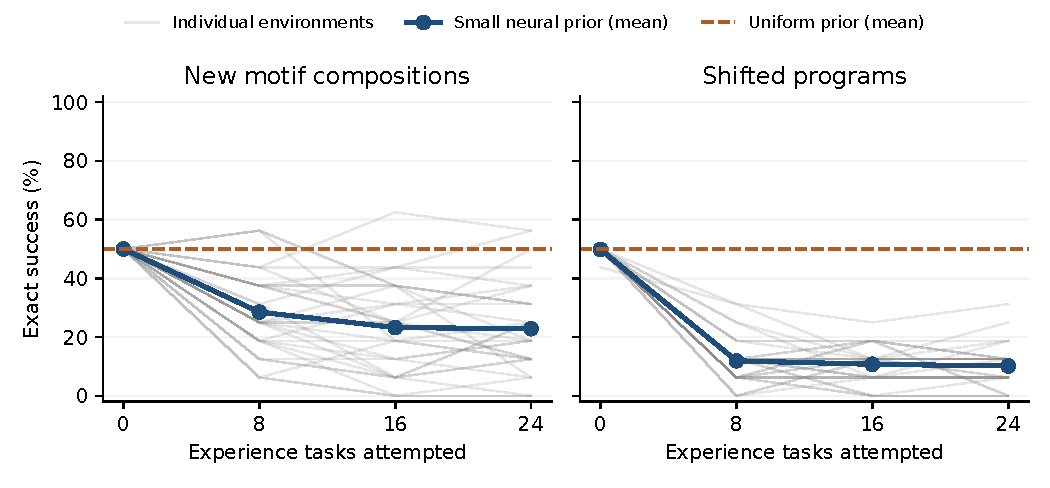
\includegraphics[width=\textwidth]{results/study-i-v1/learning-progress.pdf}
\caption{Study I small-prior transfer at the four prespecified checkpoints.
Thin lines show individual environments; the blue line shows their mean.
The zero-attempt point is the frozen initial network. The dashed reference
uses uniform search without experience. All points are scored on the same
fixed transfer tasks after training ends. Means decline in both families,
but individual trajectories vary; these descriptive curves do not imply that
each update or each environment deteriorates.}
\label{fig:i-progress}
\end{figure}

Shared experience costs 3,188,241 primitive operations. Including that cost
where applicable, standalone search totals for uniform, counts, small frozen,
small trained, small shuffled, and large trained are respectively 44.14,
46.64, 43.86, 63.64, 62.14, and 65.07 million operations. Corresponding
reconstructed phase-time sums are 2.739, 2.847, 27.705, 25.907, 25.969, and
29.562 seconds. These sums charge initialization, optimizer setup, training,
count construction, ranking, and search as applicable, using shared measured
phases; they are not separate wall-time trials or equal total computation.

Actual collection includes the intermediate probes and uses 434,569,422 search
operations. It processes 2,304,000 replay target tokens and 9,606,438 neural
prefix positions. Training takes 26.203 seconds, ranking 103.961 seconds, and
search 17.751 seconds. Full collection takes 150.076 seconds on the lens AMD
Ryzen 9 9950X CPU. Independent audit and analysis take 84.424 seconds.
The hidden evaluator adds
302,256 primitive operations outside search. All 352 checkpoint files are
retained, including optimizer states, occupying 43,789,664 archive bytes;
this is not an inference-RAM measurement. The complete 969-file raw/audit
archive matches its originals, and both intervals were independently reproduced.
No experiment source, task, seed, budget, or checkpoint selection changed after official
development or formal outcomes.

\subsection{Post-hoc experience fit and transfer likelihood}
The small trained prior lowers raw loss on the full accepted corpus relative
to its frozen state in all 32 environments. Its mean is 0.662957 nats per
token, versus 1.393215 initially: a mean difference of $-0.730258$.
The empirical prefix bound is 0.635611, with mean excess 0.027347.
This establishes improved fitting of the observed experience under the
next-token objective. It does not establish improved task-solving ability.

\begin{table}[ht]
\centering\small
\begin{tabular}{lrrr}
\toprule
Prior & Full experience & Composition & Shifted \\
\midrule
Uniform & 1.3863 & 1.3863 & 1.3863 \\
Counts & 1.0298 & 1.0913 & 1.5098 \\
Small frozen & 1.3932 & 1.3897 & 1.4000 \\
Small trained & 0.6630 & 2.5964 & 3.3573 \\
Small shuffled & 2.2551 & 2.3209 & 2.9893 \\
Large trained & 0.6473 & 2.9522 & 3.6507 \\
Small after 8 attempts & 1.4153 & 2.1319 & 2.7116 \\
Small after 16 attempts & 0.9803 & 2.4225 & 3.0870 \\
\bottomrule
\end{tabular}
\caption{Post-hoc raw next-token loss, nats per token (lower is better),
equally averaged across 32 environments. Full experience uses the same 24
real accepted programs for every row, including the shuffled and early
checkpoints. Transfer columns score the original generating sequences,
not every semantically equivalent solution. No new training occurs.}
\label{tab:i-likelihood}
\end{table}

On composition generating programs, small-trained raw loss exceeds uniform
in every environment; its mean excess is 1.210152 nats/token. The original
search smoothing reduces absolute loss to 1.824081, still 0.437787 above
uniform on average, with positive differences in 31 environments and a
negative difference in one. Shifted raw loss is 3.357285 and smoothed loss
is 2.144459; both exceed uniform in all 32 environments. Improved experience
fitting therefore coexists with unfavorable transfer likelihood and the
original lower search success. These are distinct descriptive outcomes,
not an estimate that one caused another.

The final larger network has a smaller mean experience excess over the same
bound, 0.011663, yet higher transfer loss and lower original search success
under the fixed schedule. The count prior fits real experience less closely
than the final small and large priors trained on that corpus, while assigning
higher likelihood to composition generating programs. Its shifted loss exceeds
uniform. Thus closeness to the in-sample optimum alone does not establish
transfer quality; other optimization or regularization interventions remain
untested. The shuffled learner's own-corpus loss is 0.703128, with bound
0.630918 and excess 0.072211. This differs from its loss on real experience
in Table~\ref{tab:i-likelihood}. Intermediate own-corpus losses also concern
different datasets and cannot be read as a fixed-corpus learning curve.

Every length/position cell is archived. For the small trained prior, mean
loss already exceeds uniform at positions one through five in both transfer
families and both lengths, under raw and smoothed scoring. However, content
and motif placement also differ between experience and transfer; these cells
do not isolate positional overfitting or length extrapolation as a cause.
Furthermore, the generating sequence is only one possible solution. Its
likelihood does not measure total probability over semantically equivalent
programs or exclude shorter successful candidates.

The diagnostic took 4.349 seconds on the lens CPU and retained 17,408 program
records, including duplicate views of actual training corpora. All 84,480
neural target probabilities and logs agree with independent NumPy equations
at absolute/relative tolerance $10^{-12}$. Standard-library reconstruction
on lens and locally agrees on the complete grid, 12,128 environment cells,
379 aggregates, 160 training-corpus summaries, and six paired contrasts.
All original file hashes and transferred diagnostic files match their
recorded sources. The analysis plan, source freeze, raw scores, and all
descriptions are archived separately from the original experiment.

\subsection{Study J: local context improves conditional transfer}
The local-trained prior solves 406/512 compositions (79.30\%), compared with
124/512 (24.22\%) for full-trained. The primary paired difference is
$+55.08$ percentage points, t95 [45.60,64.56] and bootstrap95 [45.90,63.87].
Thirty environments improve and two tie; the intervals agree and satisfy the
prespecified positive criterion. Full-trained itself performs below uniform,
so the size of this primary contrast must be read with its controls.

\begin{table}[ht]
\centering\small
\begin{tabular}{lrrr}
\toprule
Prior & Composition (\%) & Shifted (\%) & Balanced exact / 1,024 \\
\midrule
Uniform & 50.00 & 50.00 & 512 \\
Counts & 66.02 & 33.20 & 508 \\
Full frozen & 48.83 & 50.00 & 506 \\
Local frozen & 48.83 & 50.00 & 506 \\
Full trained & 24.22 & 12.70 & 189 \\
Local trained & 79.30 & 11.13 & 463 \\
Full after 8 attempts & 27.73 & 11.91 & 203 \\
Full after 16 attempts & 27.54 & 10.74 & 196 \\
Local after 8 attempts & 61.13 & 13.09 & 380 \\
Local after 16 attempts & 75.00 & 10.94 & 440 \\
\bottomrule
\end{tabular}
\caption{Study J exact success at 65,536 primitive executions per task,
32 fresh environments and 512 tasks per family. Both neural paths share
initial tensors, accepted experience, and update counts. The execution cap
excludes training and ranking; the balanced column combines the two families
equally. All controls and intermediate checkpoints are retained.}
\label{tab:j-results}
\end{table}

Descriptively, local-trained exceeds uniform by 29.30 points and local-frozen
by 30.47 points on compositions; each comparison has 31 positive environments
and one tie. Shifted success falls to 57/512 (11.13\%), a deficit of 38.87
points relative to either control in the aggregate, with a deficit in every
environment. Its balanced score is 463/1,024 (45.21\%), 4.79 points below
uniform: 20 environments worse, six tied, and six better. Counts also fall
short of uniform's balanced total. The primary success therefore coexists
with a distribution-specific failure, not overall superiority.

\begin{figure}[ht]
\centering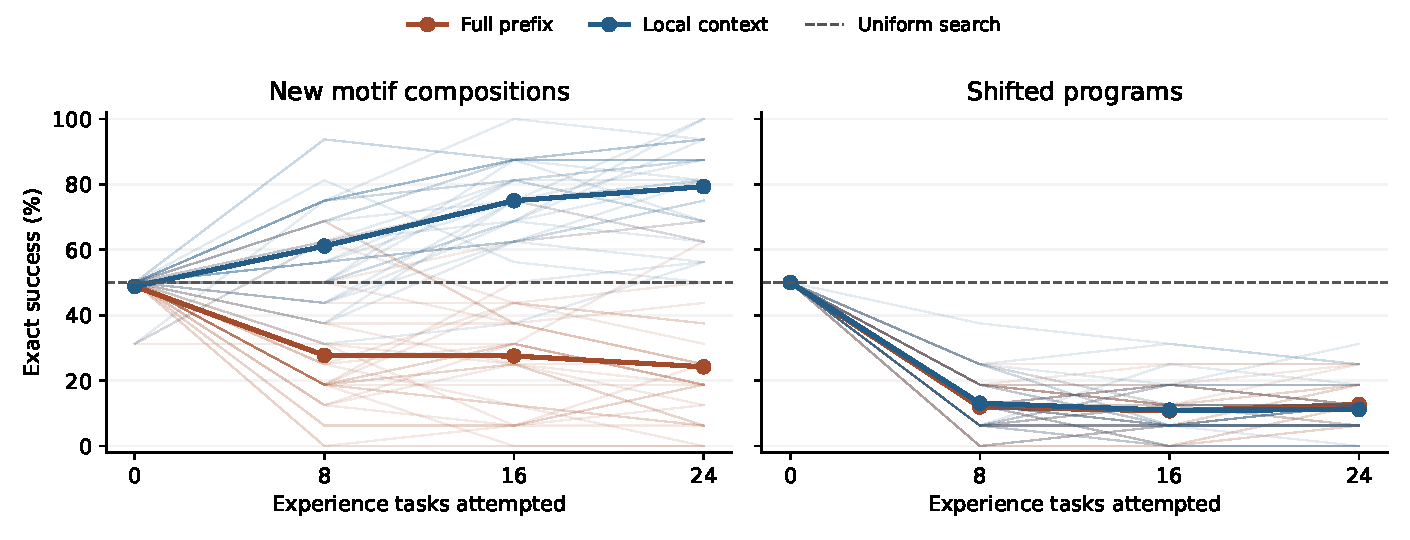
\includegraphics[width=\textwidth]{results/study-j-v1/learning-progress.pdf}
\caption{Study J transfer at every prespecified experience checkpoint.
Faint lines show individual environments; thick lines show means. Local
composition success rises through 61.13\%, 75.00\%, and 79.30\% after
8/16/24 attempts, while shifted success remains far below its initial
50.00\%. These are descriptive trajectories, not selected stopping points
or evidence of monotonic improvement in every environment.}
\label{fig:j-progress}
\end{figure}

All 768 experience solutions are exact. Across experience and transfer,
4,671 searches accept exact solutions and 6,337 exhaust the cap; no false
acceptance or skipped replay attempt occurs. Actual collection performs
11,008 searches and 24,576 gradient steps, using 1,536,000 replay target tokens.
The combined physical training input is 921,600 rows and 3,072,000 padded
positions. Ranking makes 2,390,113 prior predictions with 9,416,727 recurrent
input positions, distinct from its 18,153,098 logical full-prefix positions.

\begin{table}[ht]
\centering\small
\begin{tabular}{lrrrr}
\toprule
Final arm & Search ops & Phase seconds & Training inputs & Ranking inputs \\
\midrule
Uniform & 43,571,131 & 2.577 & 0 & 0 \\
Counts & 46,670,297 & 2.915 & 0 & 0 \\
Full frozen & 44,515,010 & 26.564 & 0 & 2,429,656 \\
Local frozen & 44,464,513 & 17.431 & 0 & 997,668 \\
Full trained & 63,289,610 & 25.095 & 768,000 & 1,414,642 \\
Local trained & 48,238,112 & 18.147 & 2,304,000 & 544,350 \\
\bottomrule
\end{tabular}
\caption{Study J standalone phase sums over 32 environments. Search includes
required experience acquisition. Training inputs count physical padded
recurrent positions; ranking inputs count actual recurrent positions.
Measured phases are shared and ranking is amortized over 32 transfer tasks,
so these are neither independent wall-time benchmarks nor equal-FLOP trials.}
\label{tab:j-costs}
\end{table}

The actual combined run, including probes, uses 499,770,365 primitive search
executions and 463,248 additional hidden-evaluation executions. Shared
experience accounts for 3,152,551 search executions. Training takes 15.519
seconds, ranking 110.839, and search 20.520; collection totals 149.137 seconds
on one AMD Ryzen 9 9950X CPU thread. Independent audit/analysis takes 74.098
seconds. All 224 checkpoint files occupy 7,333,536 bytes including optimizers,
not a measure of inference RAM. All 969 raw/audit files match the execution
host, and separate local reconstruction reproduces every seed/budget score,
descriptive contrast, and both primary intervals.

This study establishes a local-context intervention's composition benefit
under the frozen mechanism. It does not identify which changed property is
responsible, learn the restriction itself, or show that shorter contexts are
generally preferable. The same small network can yield very different
transfer when experience is represented differently, within a system whose
symbolic search and task structure remain supplied.

\subsection{Study K: continued learning improves composition reuse}
Online's final balanced score is 51.56\%, versus 43.75\% frozen. The primary
paired difference is $+7.81$ percentage points, t95 [4.74,10.88] and
bootstrap95 [4.98,10.84], with 22 positive environments, eight ties, and two
negative differences. Both intervals are positive. This satisfies the
declared primary criterion under the frozen continuation mechanism.

\begin{table}[ht]
\centering\small
\begin{tabular}{lrrr}
\toprule
Final arm & Composition (\%) & Shifted (\%) & Balanced (\%) \\
\midrule
Uniform & 50.00 & 50.39 & 50.20 \\
Frozen & 76.17 & 11.33 & 43.75 \\
Initial-corpus replay & 75.78 & 10.55 & 43.16 \\
Online accepted solutions & 92.38 & 10.74 & 51.56 \\
\bottomrule
\end{tabular}
\caption{Study K untouched probe success at 65,536 primitive executions per
 task. Each family has 256 unique tasks evaluated under two dependent stream
 orders, yielding 512 task/order conditions. The balanced mixture has 512
 unique tasks and 1,024 conditions. Frozen/uniform outcomes are measured once
 and reused. Inference uses 32 environment means, not repeated conditions.}
\label{tab:k-results}
\end{table}

Additional replay of initial experience scores 43.16\%, giving a descriptive
online-minus-replay balanced difference of $+8.40$ points: 25 environments
improve, five tie, and two decline. The observed online gain is therefore not
accounted for by the same additional update count on the initial corpus.
However, new accepted data and greater physical training work change together.
This does not isolate the effect of new feedback at equal computation.

Uniform scores 50.20\% on the balanced mixture; online's descriptive advantage
is only $+1.37$ points, with 15 positive environments, seven ties, and ten
negatives. This comparison is not a second confirmatory superiority claim.
The primary compares against a previously specialized learned model. Its
positive result is concentrated in compositions: online exceeds frozen by
16.21 points but is 0.59 points below it on shifted probes. Relative to
uniform, online gains 42.38 composition points and loses 39.65 shifted points;
the shifted deficit occurs in every environment.

\begin{table}[ht]
\centering\small
\begin{tabular}{llrrr}
\toprule
Order / arm & Attempts & Composition (\%) & Shifted (\%) & Balanced (\%) \\
\midrule
Either / common learned & 0 & 76.17 & 11.33 & 43.75 \\
Either / replay & 8 & 75.39 & 10.16 & 42.77 \\
Either / replay & 16 & 75.78 & 10.55 & 43.16 \\
Composition first / online & 8 & 92.19 & 10.55 & 51.37 \\
Composition first / online & 16 & 92.19 & 10.55 & 51.37 \\
Shifted first / online & 8 & 76.17 & 10.16 & 43.16 \\
Shifted first / online & 16 & 92.58 & 10.94 & 51.76 \\
\bottomrule
\end{tabular}
\caption{Every Study K learned checkpoint, with probes evaluated only after
 all stream learning finishes. Attempt zero is after 24 initial experience
 tasks. Frozen/uniform remain unchanged. The order changes which family
 supplies the first eight stream tasks; each block alternates lengths.}
\label{tab:k-progress}
\end{table}

\begin{figure}[ht]
\centering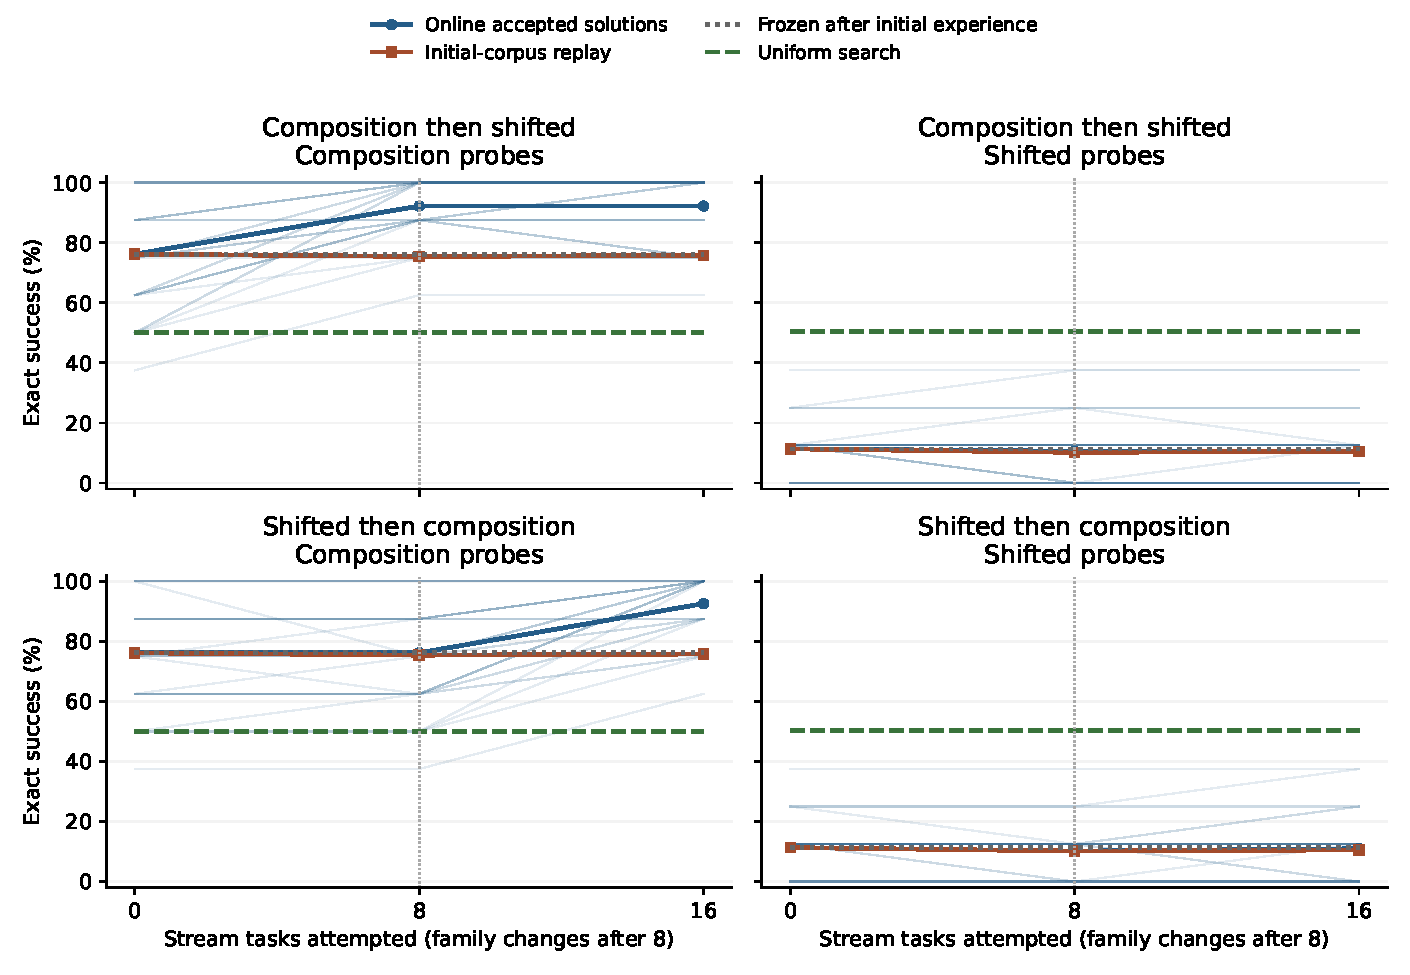
\includegraphics[width=\textwidth]{results/study-k-v1/learning-progress.pdf}
\caption{Study K untouched probe trajectories. Faint lines show all 32 online
 environment trajectories; thick lines and dashed controls show means. The
 family changes after eight stream tasks. Composition gains follow the
 composition block in either order; shifted probe success remains low.
 These are descriptive fixed checkpoints, not selected stopping points.}
\label{fig:k-progress}
\end{figure}

Composition-first online means are unchanged between attempts eight and
sixteen, but equal aggregates do not establish retention of each solved task.
Prequential stream success is recorded before each task's update: online
accepts 220/256 composition and 23/256 shifted tasks in composition-first
order, and 219/256 composition and 25/256 shifted tasks in the reverse order.
The accepted solutions are exact in this sample. Most new accepted
experience therefore comes from the motif family; no oracle supplies
solutions to exhausted searches. This describes the information available
to the update rule without isolating the cause of its shifted-task failure.

Actual collection performs 8,960 searches: 768 initial experience, 3,072 stream,
and 5,120 probes. All 4,534 acceptances are exact and 4,426 searches exhaust
their caps. No replay batch is skipped. The run performs 45,056 gradient
steps, processing 5,169,744 target tokens/rows and 15,509,232 physical padded
training positions. Its 2,080 neural tables require 43,680 model calls and
118,560 recurrent positions. Ranking constructs 2,112 orders with 11,966,349
logical queries and 94,509,370 logical prefix positions; lookup is not a
neural forward call. A table holds 672 numeric bytes excluding keys/storage
overhead; neither this nor 1,172 neural parameters measures total capacity.

\begin{table}[ht]
\centering\small
\begin{tabular}{llrrr}
\toprule
System & Order & Search executions & Training positions & Phase seconds \\
\midrule
Uniform & Either & 21,793,204 & 0 & 1.627 \\
Frozen & Either & 25,747,732 & 2,304,000 & 10.073 \\
Replay & Composition first & 25,815,114 & 5,253,120 & 16.623 \\
Replay & Shifted first & 25,815,114 & 5,253,120 & 16.469 \\
Online & Composition first & 44,012,797 & 6,233,760 & 25.255 \\
Online & Shifted first & 44,046,338 & 5,681,232 & 25.407 \\
\bottomrule
\end{tabular}
\caption{Study K final-only standalone phase sums across 32 environments.
 Necessary experience and updates are charged; replay's diagnostic stream
 searches/intermediate orders are excluded, while online needs them. Training
 positions count padding. Frozen/uniform are shared, not repeated timing trials.
 Replay timing includes step-journal writes; these are unequal lifetime costs.}
\label{tab:k-costs}
\end{table}

The complete actual run uses 353,869,176 primitive search executions and
478,640 additional hidden-evaluator executions. Shared initial experience
accounts for 3,167,190 search executions. Training takes 33.356 seconds,
table construction 2.197, ranking 31.792, and search 14.859. Collection totals
92.183 seconds on one AMD Ryzen 9 9950X CPU thread; independent audit/analysis
takes 142.827 seconds. The 320 checkpoint files occupy 11,215,168 bytes
including optimizer/corpus records, not inference RAM. All 4,586 raw/audit
files match the host. Separate local reconstruction reproduces 4,608 probe
cells, 1,536 prequential cells, 324 aggregates, nine descriptive contrasts,
and both primary intervals. Every state, order, task, and failure is retained.

\subsection{Study L: failure gradients change weights without a primary gain}
The unchanged 32-environment grid completes after the passing development
audit. Table~\ref{tab:l-success} reports exact final success. Rejection-loss
updates score 493/1,024 balanced tasks (48.14\%), versus 518/1,024 (50.59\%)
for uniformizing updates. The sole primary difference is $-2.44$ percentage
points, paired t95 [$-4.50,-0.38$] and bootstrap95 [$-4.49,-0.68$]. Both
intervals are below zero; the registered positive criterion is not met.
Rejection wins in three environments, ties in 17, and loses in 12. The four
arms share the same tasks; the 32 environment means are the inferential units.

\begin{table}[ht]
\centering\small
\begin{tabular}{lrrr}
\toprule
Arm & Composition & Shifted & Balanced \\
\midrule
Uniform & 256/512 (50.00\%) & 256/512 (50.00\%) & 512/1,024 (50.00\%) \\
Frozen & 378/512 (73.83\%) & 58/512 (11.33\%) & 436/1,024 (42.58\%) \\
Uniformizing & 262/512 (51.17\%) & 256/512 (50.00\%) & 518/1,024 (50.59\%) \\
Rejection & 258/512 (50.39\%) & 235/512 (45.90\%) & 493/1,024 (48.14\%) \\
\bottomrule
\end{tabular}
\caption{Study L final exact success at 65,536 primitive executions per task.
 The registered primary compares rejection with uniformizing on the balanced
 mixture. Families and other comparisons are descriptive; weights reset for
 every new transfer task.}
\label{tab:l-success}
\end{table}

Rejection descriptively improves over freezing by 5.57 balanced points but
trails uniform search by 1.86 points. Relative to freezing, its 34.57-point
shifted recovery accompanies a 23.44-point composition loss. Uniformizing
recovers at least as much balanced success despite ignoring rejected
identities in its loss. Recovery from a specialized prior therefore cannot
alone establish a useful effect of failure content. This comparison does not
identify the cause of rejection's deficit. No false acceptance appears in the
recorded grid, which does not certify the checker for arbitrary tasks.

Every adaptive batch changes all 1,172 parameter values. Rejection takes
178,848 Adam steps in 11,178 batches; uniformizing takes 151,280 steps in
9,455 batches. There are no skipped adaptive batches. Batch parameter-change
L2 norms are strictly positive in both arms and every tensor/optimizer state
is reconstructed by audit. Thus the negative primary is not a consequence of
omitting weight updates. Each task starts from the common learned checkpoint
with a fresh optimizer, so these updates do not establish retained cross-task
capability.

At 4,096 operations the three learned arms each score 14.16\% balanced success,
versus uniform's 0.00\%. No adaptive update has yet affected an executed
candidate at that endpoint. At 16,384 operations the corresponding scores are
25.29\% frozen, 22.95\% uniformizing, 17.58\% rejection, and 17.77\% uniform.
Figure~\ref{fig:l-success} shows all registered endpoints and final paired
differences. These lower-budget scores follow the actual full-budget learning
path, without retraining or checkpoint selection.

\begin{figure}[ht]
\centering
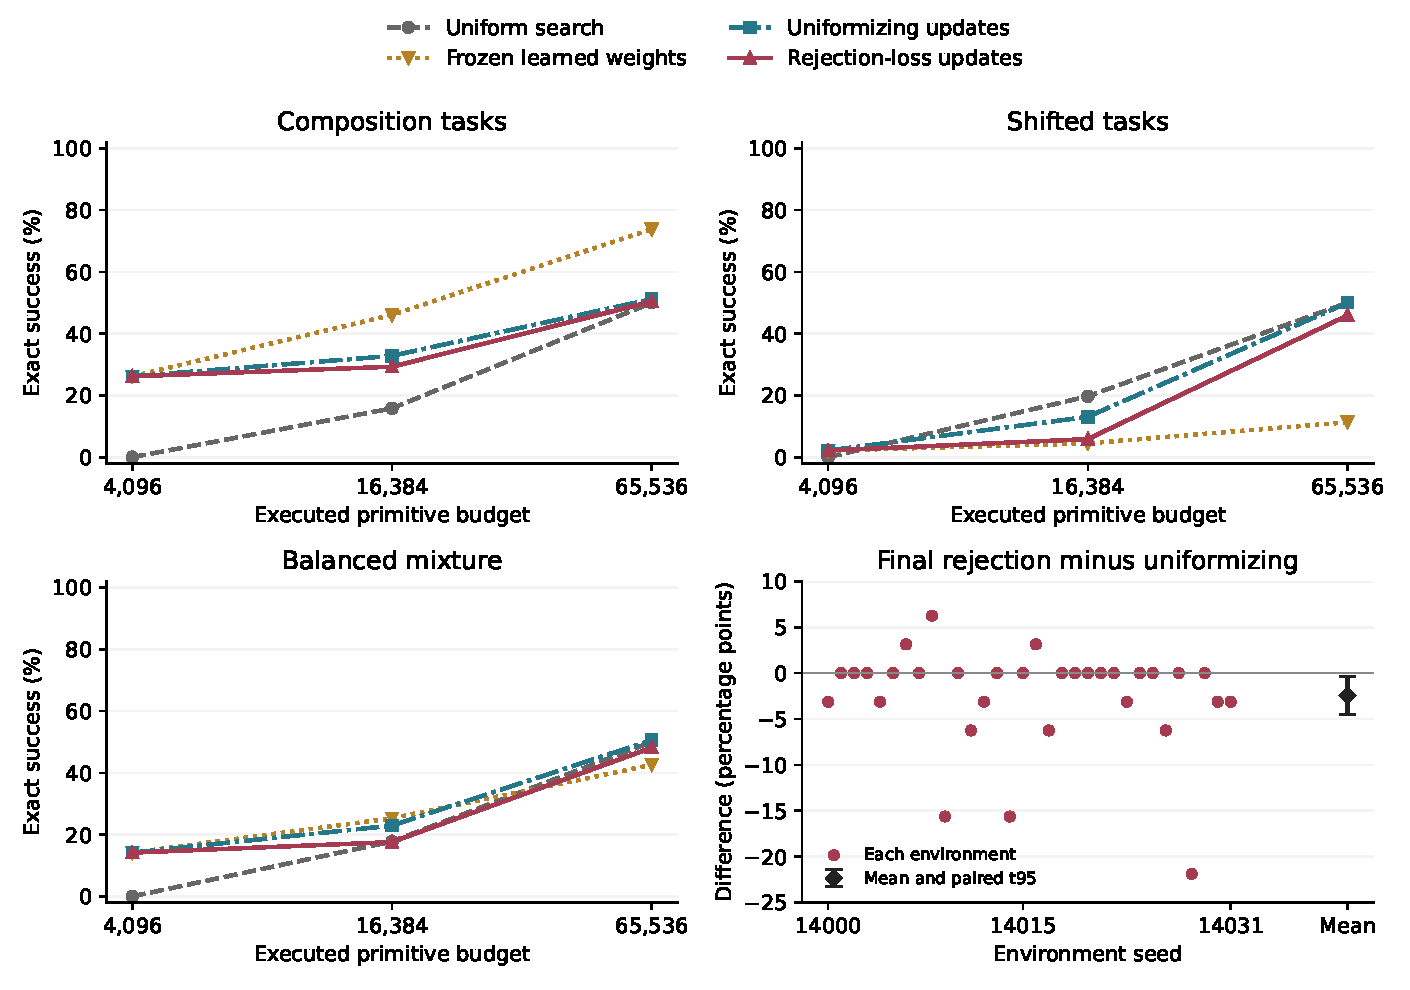
\includegraphics[width=\linewidth]{results/study-l-v1/success-and-contrasts.pdf}
\caption{Study L success at registered operation budgets and each final
 environment's rejection-minus-uniformizing difference. Curves are descriptive
 means, not continued learning across tasks. The diamond and t95 interval
 summarize the sole paired primary; the bootstrap interval is also below zero.}
\label{fig:l-success}
\end{figure}

\begin{table}[ht]
\centering\small
\begin{tabular}{lrrrr}
\toprule
Arm & Primitive executions & Gradient steps & Padded positions & Seconds \\
\midrule
Uniform & 43,948,916 & 0 & 0 & 21.907 \\
Frozen & 48,940,473 & 12,288 & 2,304,000 & 27.587 \\
Uniformizing & 45,052,778 & 163,568 & 11,834,640 & 215.281 \\
Rejection & 51,995,043 & 191,136 & 13,571,424 & 713.812 \\
\bottomrule
\end{tabular}
\caption{Study L standalone phase sums over 32 environments. Each learned arm
 includes initial acquisition and 12,288 initial gradient steps once per
 environment set; uniform needs no initial learning. Positions count physical
 training inputs including padding. Seconds include measured journal costs
 and are not independent wall-time trials or matched lifetime compute.}
\label{tab:l-costs}
\end{table}

Table~\ref{tab:l-costs} charges necessary initial learning to each standalone
learned arm while actual collection executes it once. Included journal times
are 13.913 seconds uniform, 12.420 frozen, 15.377 uniformizing, and 17.573
rejection. Rejection processes 772,391,024 rejected-program exposures and
5,073,457,216 token exposures across gradients. These count repeated loss
processing, not distinct programs or additional neural input positions.
Equal update opportunities yield unequal realized steps and objective work.

Actual collection includes 4,864 searches (768 initial and 4,096 transfer),
183,561,514 primitive executions, 257,088 hidden-evaluator executions,
342,416 gradient steps, and 25,936,224 candidate/boundary events. It takes
985.204 seconds on one AMD Ryzen 9 9950X CPU thread with float64; Study L does
not use the server GPU. Independent audit/analysis takes 688.739 seconds.
All 25,529 checkpoint files occupy 863,577,169 bytes, an accumulated research
archive rather than inference RAM. The 73,076 transferred raw/audit files,
totaling 5,442,329,227 bytes, match the host, including all 73,074 audited raw
files. Separate local reconstruction reproduces 1,152 outcome cells,
36 aggregates, nine contrasts, both primary intervals, and 128 standalone
cost cells. All failed searches and intermediate states remain archived.

\subsection{Study M: retained predictive weights do not favor the smaller model}
Study M evaluates the registered retained-learning intervention on 32 formal
seeds, each with structured and random worlds. The audit reconstructed 262,144
main actions, 665,600 gradient steps, 2,816 model/optimizer/replay checkpoints,
and 444,416 fixed-graph probe tasks. All 64 formal worlds passed the frozen generator
checks; the independent replay matched every action, gradient, Adam state,
checkpoint, and probe record. All 69,632 immediate and delayed adaptive batches
changed at least one parameter value. These are implementation facts, not
success guarantees.

The sole primary is the structured-world AUC difference between small immediate
and large immediate branches. The small model's AUC is 0.9143 and the large
model's 0.9168, for a difference of $-0.247$ percentage points. The paired
95\% $t$ interval is $[-1.128,0.633]$ points and the 10,000-sample bootstrap
interval is $[-1.081,0.569]$ points. Sixteen of 32 seed differences favor each
branch. The pre-registered lower bound is not above zero, so the primary does
not support small-model superiority; the interval does not establish
equivalence.

Both immediate branches improve sharply from their frozen initializations in
these structured worlds. Small success rises from 23.22\% at the initial
checkpoint to 100.00\% after 512 interactions; large success rises from
22.73\% to 100.00\%. The corresponding AUCs are 0.9143 and 0.9168, while
frozen branches remain at their initial 23.22\% and 22.73\%. Delayed updates
reach the same final success but have AUCs 0.8963 (small) and 0.8948 (large).
The exact observed-table control reaches 96.37\% at the final probe and has
AUC 0.8817; uniform action remains at 21.57\% with AUC 0.2157. Thus the
learning curves show useful predictive adaptation in this structured domain,
but the primary does not separate the 485-parameter learner from the
1,925-parameter learner in favor of the smaller one.

Random worlds are harder and show the same capacity qualification. Small and
large immediate branches finish at 85.22\% and 97.09\%, with AUCs 0.6752 and
0.7153. Delayed branches finish at 86.48\% and 96.89\%; the observed table
reaches 96.98\%, and uniform action remains at 22.43\%. The random-world
curves are descriptive because the sole primary was registered on structured
worlds. Every true-graph probe in both families is within the eight-action cap
in this generated grid, so the supplied shortest-path bound does not explain
away the learning curves.

\begin{figure}[ht]
\centering
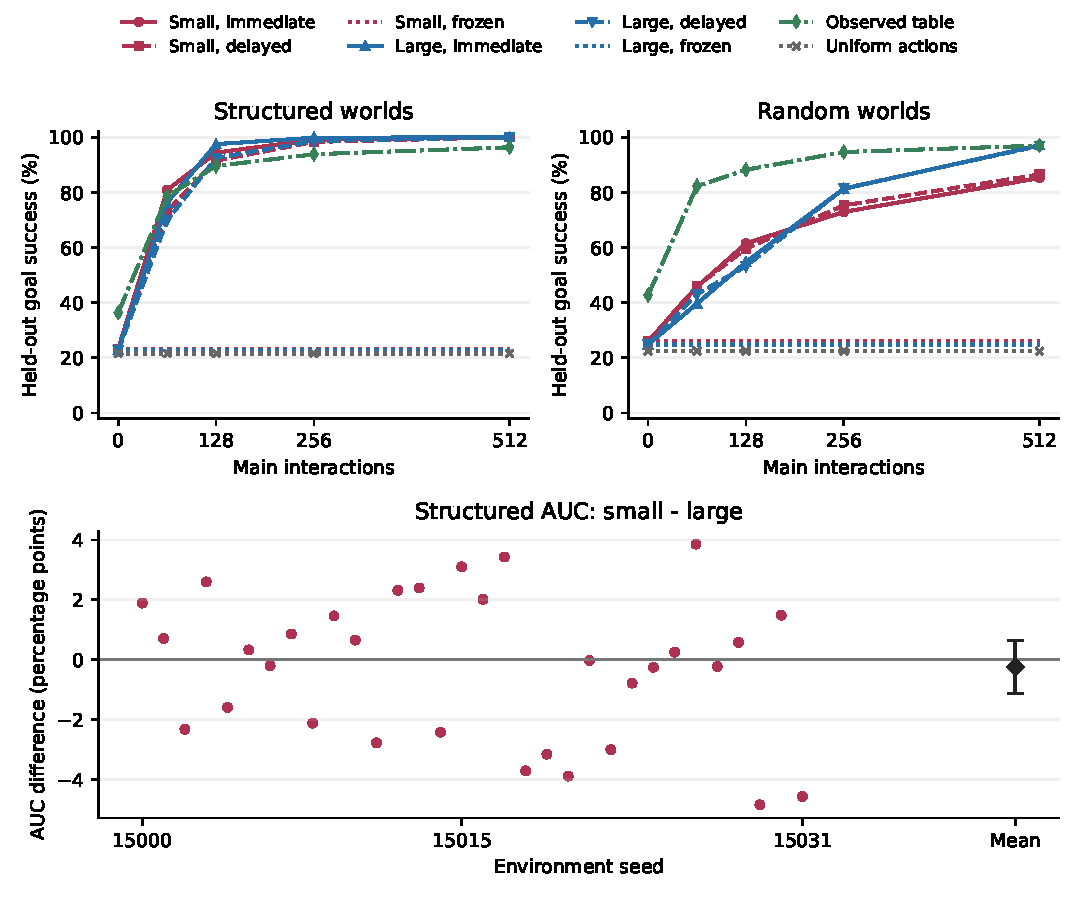
\includegraphics[width=\linewidth]{results/study-m-v1/learning-and-contrasts.pdf}
\caption{Study M held-out-goal learning curves at every fixed checkpoint,
averaged over 32 paired environments. Curves are descriptive. The lower panel
shows the registered structured-world small-minus-large AUC difference for
each seed and its paired mean with a 95\% $t$ interval. The zero-spanning
interval establishes neither small-model superiority nor equivalence.}
\label{fig:m}
\end{figure}

The training matrix proxy is matched per observed transition: 270,336 dense
training MACs for either immediate width allocation. Full work differs. Across
both families and all formal seeds, small immediate consumes 270,336 gradient
steps and 9.135 billion training MACs, while large immediate consumes 67,584
steps and the same proxy MAC total; their dense graph-forward totals are
1.883 and 7.531 billion MACs. Collection records 236.9 seconds, 2,463,567
physical actions, 964,917,075 journal bytes, and 74,892,864 checkpoint bytes.
Collection uses the lens AMD Ryzen 9 9950X CPU; its GPU is not used.
Independent audit and analysis take 322.529 seconds. These figures include
archive and probe work in actual totals; standalone
learned-arm costs charge shared warmup and initialization once and exclude
archive-only graph writes.

Study M therefore establishes the narrower result that a very small model can
learn an actionable transition predictor from dense action outcomes and retain
it while pursuing new goals in a fixed domain. It does not establish that
feedback alone is sufficient, that the smaller model is generally as capable,
or that the supplied representation, replay memory, planner, and stationary
world can be removed. The controller observes its current true state even in
frozen probes, and held-out goals are new goal cues rather than new dynamics.
\subsection{Limitations and interpretation}
All thirteen studies use synthetic tasks with disclosed families and inexpensive
feedback. They do not measure open-ended exploration, long-horizon reward,
human intelligence, or general cross-domain skill accumulation. Study A's
fixed optimization schedule may interact with capacity. Its replay treatment
also changes fresh-example exposure. Study B uses only one model family and
a first-token response interface. Study C adds full generation but also a
strict final-line format and a fixed token cap. Study D shows that extending that cap can materially
change accuracy with the same prompt and model. Study E tests only 16 online
outcomes and reuses the narrow first-token interface; it is not an optimized
learning algorithm or a full-generation test. Low accuracy can reflect the
interface, instruction-following ability, prior execution ability, or the
specific update schedule. Study F adds error-directed rule revision with
equal call caps, but neither equal measured compute nor an open-ended
reflection agent. Its executor and disclosed rule family contribute supplied
capability, and its final score does not measure learning across languages.
Study G extends revision to 16 rounds and retains complete transcripts,
but supplies all task examples from the start and adds no new observations.
It tests transcript availability together with increased context and compute,
not a fixed-cost memory comparison. Its ungated last-proposal policy can
discard earlier success; mechanisms that preserve verified progress require
their own prospective comparisons. The 7B and other secondary contrasts are
descriptive and do not receive multiplicity adjustment.
The subsequent selection and uniform references are explicitly post-hoc.
Their known grammar and full-example scorer supply capability, and a
conditional policy expectation is not a measured random-agent outcome or
an interactive intervention. They do not establish general intelligence
through random search or through retaining the best synthetic-task candidate.

Study H deliberately creates shared motifs and tests only one frozen
experience-to-transfer cycle. The searcher, primitive tables, flat compression
algorithm, task-generation structure, and exact checker are supplied. Whole
and compressed memory differ in vocabulary size and storage; the renamed
control addresses content at matched entry lengths but does not create a
universal memory baseline. The primitive-operation cap excludes other work,
and prior experience differs from the no-memory arm. A favorable primary
contrast therefore does not establish improved general intelligence, a neural
capacity threshold, or overall superiority across the tested distributions.
Hierarchical abstraction, evolving neural search policies, noisy feedback,
and continual library updates are outside this experiment.

Study I learns an unconditional program prior from length-five solutions
obtained by a supplied searcher, then transfers to lengths six and nine.
Next-token fitting and successful synthesis are different objectives; the
network never receives the task's input/output examples or updates from its
failed transfer proposals. The result does not isolate architecture,
optimization, positional overfitting, or objective/distribution mismatch as
the cause. Those explanations need separate interventions. The two hidden
widths and single update schedule do not establish what an optimized or
task-conditioned learner could achieve. This is one experience-to-transfer
cycle with sequential replay, not lifelong learning or a test of all feedback
systems. The subsequent likelihood diagnostics are post-hoc descriptions of
fixed checkpoints. Their experience bounds apply in sample, and their transfer
scores use single generating sequences rather than semantic solution classes;
they identify no causal mechanism. The count comparator has a different representation and storage;
none of these comparisons equates neural parameters with total system capacity.

Study J supplies a last-two-token context and resets state at every prediction.
Its positive composition primary contrasts against a poorly transferring
full-prefix learner. Descriptive gains over uniform and local-frozen provide
additional context, while the shifted and balanced deficits limit any wider
claim. Truncation, reset, gradient paths, and physical work change together;
the experiment does not isolate positional overfitting or establish that the
context restriction is optimal. Both models still lack task-conditioned
prediction, transfer-time adaptation, and an autonomously learned memory rule.

Study K adds actual weight updates between stream tasks, with persistent
optimizer state and a separate set of untouched probes. This differs from
retaining text or changing only search memory. However, it remains a short
two-block experiment. Failures trigger additional replay without a new
corrective target; only accepted solutions supply new supervised targets.
The observed composition gain does not demonstrate shifted-family adaptation.
The positive primary is relative to a specialized frozen model, while its
small descriptive balanced advantage over uniform is not a second primary
claim. Initial acquisition, growing replay, table construction, and search
are unequal lifetime resources. Autonomous representation discovery and
failure-directed updates remain untested in this mechanism.

Study L supplies direct failure gradients within each task, but its rejection
objective penalizes mass on known failed strings rather than representing why
they failed or predicting a correct program. Finite Adam updates need not
reduce that mass monotonically. Shared local token factors can
also alter untested solutions. It does not learn primitive semantics or a
task encoder, and reset weights do not retain improvements across goals.
The negative primary applies to the fixed objective, optimizer, local prior,
schedule, and domain. It rules out neither other failure signals nor stronger
online learners. Uniformizing controls for flattening a specialized prior,
but does not match gradient scale, realized update counts, or loss work.
Its comparable recovery limits attribution of gains over freezing to useful
failure content; it does not identify the cause of rejection's deficit.
No new primary was selected after seeing the outcome. Across these sequential
studies, intervals apply to each registered comparison, not a globally adjusted
claim over the entire adaptive research program.

Study M retains predictive weights across goals, but resets them for each
world and observes exact, fully visible, stationary transitions. Its small
architecture can represent every structured world by construction; this does
not prove capacity for arbitrary random tables. Both the state encoding and
planner are supplied. Success at new goal cues does not establish learning
new dynamics, retention across unrelated domains, autonomous representation
discovery, or robust learning with noisy/delayed observations. The predictor
learns from observed transitions; it is not a general policy or language model.
The small-model budget buys four times as many Adam steps for equal dense
training-matrix MACs, while total work remains unequal. Its primary interval
does not establish equivalence, and fixed final 100\% scores in structured
worlds cannot establish equality outside this finite probe set.

In development, 0.5B answered a simple arithmetic question incorrectly under
a one-digit instruction. The official weight SHA-256 matched, and CPU float32,
GPU float32/bfloat16, and eager/SDPA paths reproduced it. A subsequent ordinary
question produced the correct answer; other ordinary-language responses were
coherent. Thus the calibration reveals prompt sensitivity, not general
arithmetic incapacity. Model files and device agreement alone cannot certify
that a response interface makes full use of the available capability.

The initial Study A random-stream defect and the corrected fresh-seed
replication are both disclosed and preserved. A disk-full error occurred only
during Study B export; every original run had completion metadata and complete
predictions. Export was repeated on a separate filesystem without rerunning
models. Study F's first 7B development load failed on a cache metadata write
to that full filesystem, before inference; its provenance and traceback are
preserved. The same frozen source and cached weights passed after enabling
offline cache access. Source hashes and complete outcome grids were checked
before analysis.

Prior work already establishes reinforcement learning, external memory,
verbal reflection, and test-time computation as relevant mechanisms. Our
current evidence is a diagnostic investigation of the stated hypothesis, not
a first discovery of feedback-driven intelligence. Targeted review of eleven
close precedents strengthens the comparison, but a systematic novelty review
remains incomplete. Studies F and G test a small structured external rule.
Study H tests one finite experience-to-transfer cycle with supplied symbolic
search and compression; Study I adds sequentially learned program priors,
Study J tests a supplied history restriction, and Study K continues neural
updates through two task-family blocks with untouched transfer probes.
Study L adds task-local failure gradients without retained cross-task updates.
Study M adds action-dependent observations and retained transition learning
across goals within a fixed world. This uses conventional predictive modeling
and supplied planning, without a claim of a new learning principle.
Open-ended abstraction learning, autonomous exploration beyond these supplied
finite worlds, retention across changing dynamics, and long-horizon reward
learning remain untested.

Stability is partially measured by Study A's old-rule retention and F/G's
within-language rule regressions. Long-term memory interference across tasks
remains untested. Our exact
synthetic targets do not reproduce the difficulty of obtaining trustworthy
real-world feedback. No study tests reward hacking: optimizing a proxy evaluator
can improve its score without improving the intended task, particularly if the
agent can influence the feedback source. These mechanisms require separate
held-out evaluation and feedback-quality experiments; faster updates alone do
not address them.

\section{Conclusion}
Feedback enables substantial adaptation in small neural learners under task
change, but capacity remains consequential when both small and large models
learn. In the smallest pretrained model, our example-conditioning and limited
parameter-update protocols do not establish compositional improvement. Its
format failures under Study C's prompt remain unresolved; Study F's new
structured interface produces mostly valid rules but no exact 0.5B recovery.
In 7B, supplying correct examples yields
substantial compositional accuracy once the continuation budget permits most
responses to finish. The earlier short-budget failures therefore cannot support
a general conclusion that this model cannot learn the disclosed rules in context.
An explicit one-pass feedback loop in the 0.5B model yields no demonstrated
compositional gain, whether it updates after every outcome or only after an
error. Retaining behavior changes therefore cannot be equated with accumulating
useful, transferable skill. External rule storage and exact example checks
also yield no demonstrated 0.5B composition gain over two self-revisions.
The larger model recovers some full rules, while retaining substantial
uncertainty and query-level regressions. Extending checked revision to 16
rounds and retaining all earlier corrections does not establish improved
0.5B direct accuracy, despite substantially greater input cost. In 7B,
increased final exact-rule counts coexist with losses of initially correct
rules. Neither additional iterations nor a complete transcript ensures
cumulative improvement under the tested update mechanism.

Post-hoc analysis exposes two distinct limits: exact candidates can appear
and then be discarded, or never appear in the recorded pool. A supplied
training-example selector recovers 17/48 full-history 7B rules, but none in
0.5B. The smaller model's selected direct score also falls below the exact
expectation of a uniform legal-proposal reference under the same supplied
selector. This comparison includes an externally specified grammar and
unequal checking costs; it does not establish a general model-size threshold.
Available candidates, retention, verification, and supplied algorithms must
therefore remain separate from claims about neural learning.

The symbolic transfer experiment adds a conditional positive mechanism:
compressing accepted solutions into reusable fragments greatly improves search
on new compositions of shared motifs, compared with storing entire solutions.
The same library reduces success on shifted random programs relative to
search without memory. This is experience-derived representation learning
implemented by a supplied symbolic algorithm, with no neural update. It shows
why external knowledge and task structure belong in a complete account of
system capability, while providing no evidence that feedback alone can replace
either inductive bias or a capable learning mechanism.

Sequential neural fitting provides a further counterexample to guaranteed
cumulative progress under a feedback mechanism: the small program prior's
new-composition score falls below uniform search despite exact accepted
experience and persistent updates. A simple count rule uses that experience
more successfully on compositions in this grid, yet loses performance after
the program distribution changes and does not exceed uniform search on the
balanced mixture. The objective, representation, transfer distribution, and
supplied search therefore remain central parts of the explanation. This
comparison does not rule out more effective small agents or update rules.
Post-hoc likelihood diagnostics confirm that improved fitting of accepted
experience can coexist with lower likelihood on transfer generating programs.
The small and large learned priors approach the unrestricted empirical
prefix-loss bound on their training corpus, yet fail to improve the original
transfer-search endpoint. These observations motivate interventions on how
experience is represented and used; they do not isolate a remedy or imply
that a different learning mechanism must fail.

The fresh local-context intervention demonstrates one conditional improvement:
with the same 1,172-parameter network, accepted programs, and update counts,
composition success reaches 79.30\% rather than 24.22\% for full-prefix
learning. This result rejects a blanket reading of the preceding failure as
incapacity of that small network. However, 11.13\% shifted success and a
balanced total below uniform search show that improved reuse remains tied
to the task distribution. The supplied history restriction and search system
are part of the mechanism, and matched parameters do not mean matched compute.

Continued learning then improves the same local prior's untouched balanced
score by 7.81 points over freezing, with a positive paired interval. The
extra-replay control does not show the same gain. Actual model parameters
change between stream tasks, but new targets arrive only from accepted
solutions. Composition success rises to 92.38\% while shifted success remains
10.74\%. The experiment supports a short continued-learning mechanism whose
benefits depend on available successful experience. This motivates the
subsequent direct test of failure-driven weight updates.

That direct intervention changes weights after verified failures during
search, yet reduces balanced success by 2.44 points relative to uniformizing
updates. It improves over the specialized frozen starting point while
remaining below uniform search descriptively. The loss discourages observed
failures without identifying the correct untested programs, and weights reset
for each goal. Thus genuine parameter updates, current-task improvement, and
retained general capability are different outcomes. This negative result
constrains one proposed mechanism; it does not settle the broader feedback
hypothesis or justify increasing the update rate without a better objective.

Study M supplies the clearest positive evidence in this version for the
narrow mechanism under test: a 485-parameter transition predictor changes its
weights after action outcomes, carries those weights through goal episodes, and
improves held-out-goal success in a stationary finite world. The registered
small-minus-large primary is slightly negative with an interval spanning zero,
so the experiment does not show that reducing parameters improves learning.
Its external state encoding, replay table, BFS planner, dense feedback, and
same-world transfer define a capable system around the predictor. The result
supports continued study of feedback efficiency while rejecting a leap from
within-domain adaptation to feedback sufficiency or unrestricted intelligence.

The supported conclusion is conditional: feedback, representation, prior
learning, update rules, and response interfaces jointly determine measured
adaptation. A strong claim about small agents needs evidence of sustained
error-directed updates, retention, and transfer across diverse tasks under
comparable resource constraints. The present study establishes neither that
feedback alone explains intelligence nor that increasing model capacity is an
incorrect research direction.

\begingroup\small
\begin{thebibliography}{11}
\bibitem{experience} D. Silver and R. S. Sutton. Welcome to the Era of Experience.
Book-chapter preprint, 2025. Author-linked copy:
\url{https://www.davidsilver.uk/publications/}.
\bibitem{silver} D. Silver, S. Singh, D. Precup, and R. S. Sutton.
Reward is enough. Artificial Intelligence, 299:103535, 2021.
\url{https://doi.org/10.1016/j.artint.2021.103535}.
\bibitem{vaswani} A. Vaswani et al. Attention Is All You Need. NeurIPS, 2017.
\url{https://arxiv.org/abs/1706.03762}.
\bibitem{kaplan} J. Kaplan et al. Scaling Laws for Neural Language Models. 2020.
\url{https://arxiv.org/abs/2001.08361}.
\bibitem{hoffmann} J. Hoffmann et al. Training Compute-Optimal Large Language Models. 2022.
\url{https://arxiv.org/abs/2203.15556}.
\bibitem{chen} H. Chen et al. Feedback is all you need: from ChatGPT to autonomous driving. 2023.
\url{https://doi.org/10.1007/s11432-023-3740-x}. Bibliographic metadata verified;
full-text argument not assessed in this version.
\bibitem{duan} Y. Duan et al. RL$^2$: Fast Reinforcement Learning via Slow Reinforcement Learning. 2016.
\url{https://arxiv.org/abs/1611.02779v2}.
\bibitem{laskin} M. Laskin et al. In-context Reinforcement Learning with Algorithm Distillation. 2022.
\url{https://arxiv.org/abs/2210.14215}.
\bibitem{shinn} N. Shinn et al. Reflexion: Language Agents with Verbal Reinforcement Learning. 2023.
\url{https://arxiv.org/abs/2303.11366v4}.
\bibitem{madaan} A. Madaan et al. Self-Refine: Iterative Refinement with Self-Feedback. 2023.
\url{https://arxiv.org/abs/2303.17651v2}.
\bibitem{huang} J. Huang et al. Large Language Models Cannot Self-Correct Reasoning Yet. ICLR, 2024.
\url{https://arxiv.org/abs/2310.01798v2}.
\bibitem{snell} C. Snell et al. Scaling LLM Test-Time Compute Optimally can be More Effective than Scaling Model Parameters. 2024.
\url{https://arxiv.org/abs/2408.03314}.
\bibitem{voyager} G. Wang et al. Voyager: An Open-Ended Embodied Agent with Large Language Models. 2023.
\url{https://arxiv.org/abs/2305.16291v2}.
\bibitem{selfdebug} X. Chen et al. Teaching Large Language Models to Self-Debug. 2023.
\url{https://arxiv.org/abs/2304.05128v2}.
\bibitem{dreamcoder} K. Ellis et al. DreamCoder: Growing generalizable,
interpretable knowledge with wake-sleep Bayesian program learning. 2020.
\url{https://arxiv.org/abs/2006.08381v1}.
\bibitem{expel} A. Zhao et al. ExpeL: LLM Agents Are Experiential Learners. 2024.
\url{https://arxiv.org/abs/2308.10144v3}.
\bibitem{unlikelihood} S. Welleck, I. Kulikov, S. Roller, E. Dinan,
K. Cho, and J. Weston. Neural Text Generation with Unlikelihood Training.
2019. arXiv v2; the PDF stylizes the title as ``DeGeneration.''
\url{https://arxiv.org/abs/1908.04319v2}.
\end{thebibliography}
\endgroup
\end{document}
